
%% One page layout:
% Margins: left 40mm, rigt 25mm, top and bottom 25mm
% (latex adds extra 1in)
\documentclass[12pt,a4paper]{report}
\setlength\textwidth{145mm}
\setlength\textheight{247mm}
\setlength\oddsidemargin{15mm}
\setlength\evensidemargin{15mm}
\setlength\topmargin{0mm}
\setlength\headsep{0mm}
\setlength\headheight{0mm}
% \openright zařídí, aby následující text začínal na pravé straně knihy
\let\openright=\clearpage

%% Two pages layout:
% \documentclass[12pt,a4paper,twoside,openright]{report}
% \setlength\textwidth{145mm}
% \setlength\textheight{247mm}
% \setlength\oddsidemargin{15mm}
% \setlength\evensidemargin{0mm}
% \setlength\topmargin{0mm}
% \setlength\headsep{0mm}
% \setlength\headheight{0mm}
% \let\openright=\cleardoublepage

\usepackage[utf8]{inputenc}
\usepackage{graphicx}
\usepackage{amsthm}

\usepackage[unicode]{hyperref}   % Musí být za všemi ostatními balíčky
\hypersetup{pdftitle=Implementing control flow resolution in dynamic language}
\hypersetup{pdfauthor=Štěpán Šindelář}

%%% Small styling hacks

% Tato makra přesvědčují mírně ošklivým trikem LaTeX, aby hlavičky kapitol
% sázel příčetněji a nevynechával nad nimi spoustu místa. Směle ignorujte.
\makeatletter
\def\@makechapterhead#1{
  {\parindent \z@ \raggedright \normalfont
   \Huge\bfseries \thechapter. #1
   \par\nobreak
   \vskip 20\p@
}}
\def\@makeschapterhead#1{
  {\parindent \z@ \raggedright \normalfont
   \Huge\bfseries #1
   \par\nobreak
   \vskip 20\p@
}}
\makeatother

% Toto makro definuje kapitolu, která není očíslovaná, ale je uvedena v obsahu.
\def\chapwithtoc#1{
\chapter*{#1}
\addcontentsline{toc}{chapter}{#1}
}




\usepackage[usenames,dvipsnames,svgnames,table]{xcolor}
\usepackage{mdframed}
\usepackage{amsfonts}
\usepackage{amsmath}
\usepackage{rotating}
\usepackage{multirow}
\usepackage{proof}
% compressed versions of listings, e.g. begin{itemize*} instead of \begin{itemize}
\usepackage{mdwlist}

\newcommand{\question}[1] {
    \begin{mdframed}
        \emph{\large{#1}}
    \end{mdframed}
}

\renewcommand{\note}[1]{\textcolor{gray}{\emph{#1}}}

\newcommand{\code}{\texttt}
\newcommand{\filepath}{\path}




% ------------------- Pygmentize

\usepackage{fancyvrb}
\usepackage{color}

\makeatletter
\def\PY@reset{\let\PY@it=\relax \let\PY@bf=\relax%
    \let\PY@ul=\relax \let\PY@tc=\relax%
    \let\PY@bc=\relax \let\PY@ff=\relax}
\def\PY@tok#1{\csname PY@tok@#1\endcsname}
\def\PY@toks#1+{\ifx\relax#1\empty\else%
    \PY@tok{#1}\expandafter\PY@toks\fi}
\def\PY@do#1{\PY@bc{\PY@tc{\PY@ul{%
    \PY@it{\PY@bf{\PY@ff{#1}}}}}}}
\def\PY#1#2{\PY@reset\PY@toks#1+\relax+\PY@do{#2}}

\expandafter\def\csname PY@tok@il\endcsname{\def\PY@tc##1{\textcolor[rgb]{0.40,0.40,0.40}{##1}}}
\expandafter\def\csname PY@tok@kt\endcsname{\def\PY@tc##1{\textcolor[rgb]{0.69,0.00,0.25}{##1}}}
\expandafter\def\csname PY@tok@kr\endcsname{\let\PY@bf=\textbf\def\PY@tc##1{\textcolor[rgb]{0.00,0.50,0.00}{##1}}}
\expandafter\def\csname PY@tok@kp\endcsname{\def\PY@tc##1{\textcolor[rgb]{0.00,0.50,0.00}{##1}}}
\expandafter\def\csname PY@tok@mi\endcsname{\def\PY@tc##1{\textcolor[rgb]{0.40,0.40,0.40}{##1}}}
\expandafter\def\csname PY@tok@mh\endcsname{\def\PY@tc##1{\textcolor[rgb]{0.40,0.40,0.40}{##1}}}
\expandafter\def\csname PY@tok@vg\endcsname{\def\PY@tc##1{\textcolor[rgb]{0.10,0.09,0.49}{##1}}}
\expandafter\def\csname PY@tok@s2\endcsname{\def\PY@tc##1{\textcolor[rgb]{0.73,0.13,0.13}{##1}}}
\expandafter\def\csname PY@tok@s1\endcsname{\def\PY@tc##1{\textcolor[rgb]{0.73,0.13,0.13}{##1}}}
\expandafter\def\csname PY@tok@vc\endcsname{\def\PY@tc##1{\textcolor[rgb]{0.10,0.09,0.49}{##1}}}
\expandafter\def\csname PY@tok@kd\endcsname{\let\PY@bf=\textbf\def\PY@tc##1{\textcolor[rgb]{0.00,0.50,0.00}{##1}}}
\expandafter\def\csname PY@tok@kc\endcsname{\let\PY@bf=\textbf\def\PY@tc##1{\textcolor[rgb]{0.00,0.50,0.00}{##1}}}
\expandafter\def\csname PY@tok@kn\endcsname{\let\PY@bf=\textbf\def\PY@tc##1{\textcolor[rgb]{0.00,0.50,0.00}{##1}}}
\expandafter\def\csname PY@tok@ow\endcsname{\let\PY@bf=\textbf\def\PY@tc##1{\textcolor[rgb]{0.67,0.13,1.00}{##1}}}
\expandafter\def\csname PY@tok@vi\endcsname{\def\PY@tc##1{\textcolor[rgb]{0.10,0.09,0.49}{##1}}}
\expandafter\def\csname PY@tok@m\endcsname{\def\PY@tc##1{\textcolor[rgb]{0.40,0.40,0.40}{##1}}}
\expandafter\def\csname PY@tok@cm\endcsname{\let\PY@it=\textit\def\PY@tc##1{\textcolor[rgb]{0.25,0.50,0.50}{##1}}}
\expandafter\def\csname PY@tok@ge\endcsname{\let\PY@it=\textit}
\expandafter\def\csname PY@tok@gd\endcsname{\def\PY@tc##1{\textcolor[rgb]{0.63,0.00,0.00}{##1}}}
\expandafter\def\csname PY@tok@gi\endcsname{\def\PY@tc##1{\textcolor[rgb]{0.00,0.63,0.00}{##1}}}
\expandafter\def\csname PY@tok@nc\endcsname{\let\PY@bf=\textbf\def\PY@tc##1{\textcolor[rgb]{0.00,0.00,1.00}{##1}}}
\expandafter\def\csname PY@tok@go\endcsname{\def\PY@tc##1{\textcolor[rgb]{0.53,0.53,0.53}{##1}}}
\expandafter\def\csname PY@tok@c\endcsname{\let\PY@it=\textit\def\PY@tc##1{\textcolor[rgb]{0.25,0.50,0.50}{##1}}}
\expandafter\def\csname PY@tok@o\endcsname{\def\PY@tc##1{\textcolor[rgb]{0.40,0.40,0.40}{##1}}}
\expandafter\def\csname PY@tok@gs\endcsname{\let\PY@bf=\textbf}
\expandafter\def\csname PY@tok@gr\endcsname{\def\PY@tc##1{\textcolor[rgb]{1.00,0.00,0.00}{##1}}}
\expandafter\def\csname PY@tok@gp\endcsname{\let\PY@bf=\textbf\def\PY@tc##1{\textcolor[rgb]{0.00,0.00,0.50}{##1}}}
\expandafter\def\csname PY@tok@gu\endcsname{\let\PY@bf=\textbf\def\PY@tc##1{\textcolor[rgb]{0.50,0.00,0.50}{##1}}}
\expandafter\def\csname PY@tok@gt\endcsname{\def\PY@tc##1{\textcolor[rgb]{0.00,0.27,0.87}{##1}}}
\expandafter\def\csname PY@tok@gh\endcsname{\let\PY@bf=\textbf\def\PY@tc##1{\textcolor[rgb]{0.00,0.00,0.50}{##1}}}
\expandafter\def\csname PY@tok@w\endcsname{\def\PY@tc##1{\textcolor[rgb]{0.73,0.73,0.73}{##1}}}
\expandafter\def\csname PY@tok@cs\endcsname{\let\PY@it=\textit\def\PY@tc##1{\textcolor[rgb]{0.25,0.50,0.50}{##1}}}
\expandafter\def\csname PY@tok@s\endcsname{\def\PY@tc##1{\textcolor[rgb]{0.73,0.13,0.13}{##1}}}
\expandafter\def\csname PY@tok@cp\endcsname{\def\PY@tc##1{\textcolor[rgb]{0.74,0.48,0.00}{##1}}}
\expandafter\def\csname PY@tok@nd\endcsname{\def\PY@tc##1{\textcolor[rgb]{0.67,0.13,1.00}{##1}}}
\expandafter\def\csname PY@tok@ne\endcsname{\let\PY@bf=\textbf\def\PY@tc##1{\textcolor[rgb]{0.82,0.25,0.23}{##1}}}
\expandafter\def\csname PY@tok@nf\endcsname{\def\PY@tc##1{\textcolor[rgb]{0.00,0.00,1.00}{##1}}}
\expandafter\def\csname PY@tok@na\endcsname{\def\PY@tc##1{\textcolor[rgb]{0.49,0.56,0.16}{##1}}}
\expandafter\def\csname PY@tok@nb\endcsname{\def\PY@tc##1{\textcolor[rgb]{0.00,0.50,0.00}{##1}}}
\expandafter\def\csname PY@tok@sx\endcsname{\def\PY@tc##1{\textcolor[rgb]{0.00,0.50,0.00}{##1}}}
\expandafter\def\csname PY@tok@nl\endcsname{\def\PY@tc##1{\textcolor[rgb]{0.63,0.63,0.00}{##1}}}
\expandafter\def\csname PY@tok@nn\endcsname{\let\PY@bf=\textbf\def\PY@tc##1{\textcolor[rgb]{0.00,0.00,1.00}{##1}}}
\expandafter\def\csname PY@tok@no\endcsname{\def\PY@tc##1{\textcolor[rgb]{0.53,0.00,0.00}{##1}}}
\expandafter\def\csname PY@tok@ss\endcsname{\def\PY@tc##1{\textcolor[rgb]{0.10,0.09,0.49}{##1}}}
\expandafter\def\csname PY@tok@ni\endcsname{\let\PY@bf=\textbf\def\PY@tc##1{\textcolor[rgb]{0.60,0.60,0.60}{##1}}}
\expandafter\def\csname PY@tok@sr\endcsname{\def\PY@tc##1{\textcolor[rgb]{0.73,0.40,0.53}{##1}}}
\expandafter\def\csname PY@tok@nt\endcsname{\let\PY@bf=\textbf\def\PY@tc##1{\textcolor[rgb]{0.00,0.50,0.00}{##1}}}
\expandafter\def\csname PY@tok@nv\endcsname{\def\PY@tc##1{\textcolor[rgb]{0.10,0.09,0.49}{##1}}}
\expandafter\def\csname PY@tok@mo\endcsname{\def\PY@tc##1{\textcolor[rgb]{0.40,0.40,0.40}{##1}}}
\expandafter\def\csname PY@tok@si\endcsname{\let\PY@bf=\textbf\def\PY@tc##1{\textcolor[rgb]{0.73,0.40,0.53}{##1}}}
\expandafter\def\csname PY@tok@sh\endcsname{\def\PY@tc##1{\textcolor[rgb]{0.73,0.13,0.13}{##1}}}
\expandafter\def\csname PY@tok@se\endcsname{\let\PY@bf=\textbf\def\PY@tc##1{\textcolor[rgb]{0.73,0.40,0.13}{##1}}}
\expandafter\def\csname PY@tok@sd\endcsname{\let\PY@it=\textit\def\PY@tc##1{\textcolor[rgb]{0.73,0.13,0.13}{##1}}}
\expandafter\def\csname PY@tok@sc\endcsname{\def\PY@tc##1{\textcolor[rgb]{0.73,0.13,0.13}{##1}}}
\expandafter\def\csname PY@tok@sb\endcsname{\def\PY@tc##1{\textcolor[rgb]{0.73,0.13,0.13}{##1}}}
\expandafter\def\csname PY@tok@k\endcsname{\let\PY@bf=\textbf\def\PY@tc##1{\textcolor[rgb]{0.00,0.50,0.00}{##1}}}
\expandafter\def\csname PY@tok@err\endcsname{\def\PY@bc##1{\setlength{\fboxsep}{0pt}\fcolorbox[rgb]{1.00,0.00,0.00}{1,1,1}{\strut ##1}}}
\expandafter\def\csname PY@tok@bp\endcsname{\def\PY@tc##1{\textcolor[rgb]{0.00,0.50,0.00}{##1}}}
\expandafter\def\csname PY@tok@mf\endcsname{\def\PY@tc##1{\textcolor[rgb]{0.40,0.40,0.40}{##1}}}
\expandafter\def\csname PY@tok@c1\endcsname{\let\PY@it=\textit\def\PY@tc##1{\textcolor[rgb]{0.25,0.50,0.50}{##1}}}

\def\PYZbs{\char`\\}
\def\PYZus{\char`\_}
\def\PYZob{\char`\{}
\def\PYZcb{\char`\}}
\def\PYZca{\char`\^}
\def\PYZam{\char`\&}
\def\PYZlt{\char`\<}
\def\PYZgt{\char`\>}
\def\PYZsh{\char`\#}
\def\PYZpc{\char`\%}
\def\PYZdl{\char`\$}
\def\PYZhy{\char`\-}
\def\PYZsq{\char`\'}
\def\PYZdq{\char`\"}
\def\PYZti{\char`\~}
% for compatibility with earlier versions
\def\PYZat{@}
\def\PYZlb{[}
\def\PYZrb{]}
\makeatother



\begin{document}

% Trochu volnější nastavení dělení slov, než je default.
\lefthyphenmin=2
\righthyphenmin=2

%%% Titulní strana práce

\pagestyle{empty}
\begin{center}

\vfill

\centerline{\mbox{
\includegraphics{img/mq-logo.png}}}

\vspace{2cm}

{\bf\Large PROJECT REPORT}

\vfill

% Název práce přesně podle zadání
{\LARGE\bfseries Static Type Analysis of a Dynamically Typed
Programming Language}

\vfill

\begin{tabular}{rl}
Author: & Stepan Sindelar \\
\noalign{\vspace{2mm}}
Student ID: & 43600220 \\
\noalign{\vspace{2mm}}
Supervisor of the project: &  Matthew Roberts \\
\noalign{\vspace{2mm}}
Study programme: & exchange student \\
\end{tabular}

\vfill

\end{center}

\newpage
\noindent
Lorem ipsum.

\newpage
\vspace{3cm}
\begin{center}
ABSTRACT:
\end{center}

Dynamic programming languages allow to write code without type 
information and the type of variables can dynamically 
change during execution, which can be easier to use 
and suitable for fast prototyping, but at the same time 
can lead to error prone code, difficult maintenance 
and is challenging for the compilers or interpreters.

Programmers often use documentation comments to provide 
the type information. However, the correspondence of the 
documentation and the actual code is usually not checked 
by the tools.

In this thesis, we focus on one of the most popular dynamic 
programming languages: PHP. We have developed a framework 
for static analysis of PHP code as a part of the Phalanger project -- 
the PHP to .NET compiler. The framework supports any type of analysis, 
but in particular, we implemented type inference analysis with emphasis 
on discovery of possible type related errors and mismatches between 
the type documentation and the actual code.

We used a modular approach to static analysis of PHP applications, 
which is different to most of the other tools of this kind. 
The implementation was evaluated on real PHP applications and 
discovered several real errors and documentation mismatches with a good 
ratio of false positives.

\newpage

%%% Strana s automaticky generovaným obsahem diplomové práce. U matematických
%%% prací je přípustné, aby seznam tabulek a zkratek, existují-li, byl umístěn
%%% na začátku práce, místo na jejím konci.

\openright
\pagestyle{plain}
\setcounter{page}{1}
\tableofcontents

%%% Jednotlivé kapitoly práce jsou pro přehlednost uloženy v samostatných souborech
\chapter{Introduction}

    \section{Problem Description}
    Static type analysis of a dynamic language, benefits: compiler optimizations, IDE support - bug hunting analysis.

    \section{Thesis structure}
%pygmentize_options: -O startinline=True

\chapter{Analysing PHP Code}

    The PHP programming language first appeared in 1995\cite{phphist}. Over the years 
    the language has evolved and so have the ways programmers use it. 
    This project focuses on PHP version 5.5\footnote{From this point, 
    if the PHP version is not stated explicitly, it is implicitly 5.5.} 
    and the aim for the analysis 
    is to work well on PHP source code written in an object oriented style, 
    using modern PHP patterns and idioms that are described later in 
    this text. The analysis, however, should provide correct results for 
    any valid PHP code of any PHP version. We do not focus only on websites, but also on 
    PHP libraries and frameworks that by themselves do not contain 
    any PHP files that produce HTML or any other output for the user.
    
    The following section PHP Semantics describes some important parts 
    of the semantics of the PHP programming language, especially those 
    that represent a challenge for static analysis.

    Section Static Code Analysis gives a brief overview of existing 
    static analysis methods, especially Data Flow Analysis 
    (DFA)\cite{aho1985compilers}\cite{nielson1999principles}, 
    which has become a de-facto standard type of analysis for most of 
    the optimizing compilers and other more complex static analysis methods 
    are either directly based on DFA or on the ideas behind DFA. 
    This section includes references to relevant literature and 
    is not meant as a comprehensive description, but should provide a 
    context for the following section Control Flow for Phalanger Approach, 
    where we discuss how we used the existing techniques for the purposes 
    of our PHP code analysis.
    
    \section{PHP Semantics}

    \subsection{Dynamic Typing}
    In PHP, local or global variables, object fields and function or 
    method parameters are dynamically typed, which means that they 
    can hold values of completely different types at different 
    times of the execution.
    
    \subsection{Local Variables}
    Local variables in PHP do not need to be declared explicitly. 
    Instead the first usage of a variable is also its declaration. 
    If a variable's value is used before the variable got any 
    value assigned, then the interpreter generates a notice, 
    however the execution continues and value \code{null} is 
    used instead. A variable can get a value assigned to it when it 
    appears on a left hand side of an assignment or when a 
    reference to that variable is created, in which case it gets value 
    \code{null}, but no notice is generated. References are 
    discussed in one of the following subsections.

    The scope of a local variable is always its parent function not the 
    parent code block as in other languages like C or Java. 
    So in the following 
    example, the usage of variable \code{\$y} at the end 
    of the function can generate uninitialized variable notice, 
    however, if \code{\$x} was equal to \code{3}, 
    \code{\$y} will have a value although it 
    was declared in the nested code block.

%pygmentize_begin php
% function foo($x) {
%   if ($x == 3) { $y = 2; }
%   echo $y; // uninitialized variable if x != 3
% }
%pygmentize_end
\begin{Verbatim}[commandchars=\\\{\}]
 \PY{k}{function} \PY{n+nf}{foo}\PY{p}{(}\PY{n+nv}{\PYZdl{}x}\PY{p}{)} \PY{p}{\PYZob{}}
   \PY{k}{if} \PY{p}{(}\PY{n+nv}{\PYZdl{}x} \PY{o}{==} \PY{l+m+mi}{3}\PY{p}{)} \PY{p}{\PYZob{}} \PY{n+nv}{\PYZdl{}y} \PY{o}{=} \PY{l+m+mi}{2}\PY{p}{;} \PY{p}{\PYZcb{}}
   \PY{k}{echo} \PY{n+nv}{\PYZdl{}y}\PY{p}{;} \PY{c+c1}{// uninitialized variable if x != 3}
 \PY{p}{\PYZcb{}}
\end{Verbatim}
    
    \subsection{Global and Local Scope}
    PHP distinguishes two scopes for variables: global scope and 
    local scope. Local scope is a scope of local variables 
    within a user defined routine.         
    Variables that are declared 
    in global scope, that is outside of a user defined routine, 
    are available anywhere in global scope and are called 
    global variables. Global variables are also available 
    in user defined routines as long as they are imported 
    into the routine's scope using the keyword \code{global}.
    
%pygmentize_begin php
% $g1 = 1;  // global variables g1 and g2
% $g2 = 2;
% function foo() {
%   global $g1;
%   echo $g1;   // prints the value of global variable g1
%   $g2 = 4;   // sets the value of local variable g2,
%   // because global variable g2 was not imported, 
%   // its value does not change
% }
%pygmentize_end
\begin{Verbatim}[commandchars=\\\{\}]
 \PY{n+nv}{\PYZdl{}g1} \PY{o}{=} \PY{l+m+mi}{1}\PY{p}{;}  \PY{c+c1}{// global variables g1 and g2}
 \PY{n+nv}{\PYZdl{}g2} \PY{o}{=} \PY{l+m+mi}{2}\PY{p}{;}
 \PY{k}{function} \PY{n+nf}{foo}\PY{p}{()} \PY{p}{\PYZob{}}
   \PY{k}{global} \PY{n+nv}{\PYZdl{}g1}\PY{p}{;}
   \PY{k}{echo} \PY{n+nv}{\PYZdl{}g1}\PY{p}{;}   \PY{c+c1}{// prints the value of global variable g1}
   \PY{n+nv}{\PYZdl{}g2} \PY{o}{=} \PY{l+m+mi}{4}\PY{p}{;}   \PY{c+c1}{// sets the value of local variable g2,}
   \PY{c+c1}{// because global variable g2 was not imported, }
   \PY{c+c1}{// its value does not change}
 \PY{p}{\PYZcb{}}
\end{Verbatim}

    Global variables can be imported and used in any user defined 
    routine. This means that even if we know some type information 
    about a global variable's value at some point in the analysed 
    code (e.g. straight after assignment to that variable), 
    any time another user defined routine is invoked, we 
    have to take into account that the other routine can 
    change the value of the global variable even if we do not 
    pass the global variable to the invoked routine 
    as an argument passed by reference.

    \subsection{Closures}
    PHP also supports anonymous functions. An anonymous function has its 
    own scope as any other function and its local variables are not visible 
    to the scope where it was declared. Variables from the parent 
    scope are available in the closure scope only if they are 
    explicitly imported to its scope and they can be captured 
    by value or by reference. Only the later represents a 
    challenge for the analysis, because any code that can 
    access the closure can invoke it and thus change the 
    values of variables imported to the closure's scope 
    by reference. By invoking a closure, we can influence 
    the values of variables in a completely different 
    and otherwise inaccessible scope.
    
    \subsection{References}
    References in PHP are similar, but not same, as pointers 
    in the C programming language. PHP has a special 
    operator \code{=\&} (assign by reference) that turns 
    the variable on the 
    left hand side into a reference to the 
    variable on right hand side. For example \code{\$a=\&\$b}, 
    after this, any assignment 
    to \code{\$a} will in fact change the 
    value of \code{\$b} and wherever 
    the value of \code{\$a} is used (e.g. in an expression), 
    the value of \code{\$b} is used instead.
    
    The variable the reference is pointing to is determined 
    in a transitive fashion, which means that if we assign 
    by reference another reference, the new reference will 
    point to where the other reference was pointing to, 
    but the intermediate link is lost. The following example 
    illustrates this.
    
%pygmentize_begin php
% $a =& $b;       // a points to b
% $c =& $a;       // c points to where a points, that is b
% $a =& $d;       // a points to d, but c still points to b
%pygmentize_end    
\begin{Verbatim}[commandchars=\\\{\}]
 \PY{n+nv}{\PYZdl{}a} \PY{o}{=\PYZam{}} \PY{n+nv}{\PYZdl{}b}\PY{p}{;}       \PY{c+c1}{// a points to b}
 \PY{n+nv}{\PYZdl{}c} \PY{o}{=\PYZam{}} \PY{n+nv}{\PYZdl{}a}\PY{p}{;}       \PY{c+c1}{// c points to where a points, that is b}
 \PY{n+nv}{\PYZdl{}a} \PY{o}{=\PYZam{}} \PY{n+nv}{\PYZdl{}d}\PY{p}{;}       \PY{c+c1}{// a points to d, but c still points to b}
\end{Verbatim}

    \subsection{Arrays}
    Arrays in PHP do not have to be homogenous and 
    they can be indexed by either integers or strings.
    In fact, PHP arrays are hash maps rather than arrays 
    in the usual sense and that is also how they are 
    implemented internally. 
    
    String indexed heterogenous arrays are often used 
    as flexible ad-hoc structured data type. 
    Instead of defining a class 
    with required fields, one can use what would be a 
    field name as an index into an array. Such arrays 
    are usually indexed only with finite number of 
    constant string values. 
    
    In this light, it is no 
    surprise that using the subscribe operator 
    \code{[]} with string index on an object instance will 
    access the field with the same name as the index value.

    \subsection{Interesting Control Flow Structures}
    The \code{break} and \code{continue} statements with 
    optional numeric argument are supported in PHP in a 
    similar way as in other imperative programming 
    languages. There are, however, important differences 
    to be noted.
    
    Firstly, The numeric argument can be an arbitrary 
    expression in some of the older versions of PHP, in which 
    case we cannot statically determine the target of 
    the jump for the control flow resolution.
    
    Secondly, the \code{switch} statement is considered 
    a loop for the purposes of both \code{break} and 
    \code{continue}. The semantics of \code{break} 
    is intuitive. One of the meaningful use cases is to 
    break a loop from within a \code{switch} by 
    using \code{break 2}. The semantics of 
    \code{continue} statement 
    is perhaps not so intuitive: within a \code{switch} 
    it works the same way as \code{break}.
    
    \subsubsection*{Switch Statement Semantics} 
    The basic semantics of the \code{switch} statement in PHP is 
    again very similar to that of other standard imperative 
    programming languages. The \code{switch} statement in PHP 
    permits an arbitrary expression as the value to be used 
    for comparison with values of its \code{case} labels. Furthermore, 
    the values of \code{case} labels can also be arbitrary 
    expressions and because we are in a context of dynamic 
    programming language, they can again evaluate to a value 
    of any type at runtime.
    
    The switch expression is evaluated only once 
    at the beginning, and if it has an undefined value (undefined variable, 
    void function call), then the control flow goes directly 
    to the default item, without evaluating the expressions 
    in the case items. If the value is defined, then it is 
    one-by-one compared to the values that the 
    \code{case} labels evaluate to. If a \code{case} label evaluates 
    to \code{boolean} value, then it is used to decide whether to 
    jump to that \code{case} item or continue with evaluating 
    the value of the next \code{case} label. Note that the value of 
    switch expression is not compared to the \code{case} label value. 
    If a \code{case} label evaluates to a complex type (\code{object} or \code{array}), 
    it is ignored and evaluation continues with the next \code{case} label. 
    And finally, if a \code{case} label evaluates to an 
    \code{integer}, \code{float} or \code{string} value, it is 
    compared to the switch expression. All these expressions can 
    have side effects due to usage of assignments as expressions 
    or calls of functions with side effects. 
    
    PHP also permits placing the \code{default} label anywhere in between 
    the other \code{case} labels. This can be used for fall-back 
    to or from a \code{case} item as in the following code sample 
    that is abbreviated version of actual code taken from the 
    WordPress\cite{wordpress} code base.
    
%pygmentize_begin php
%switch ( $status ) {
%    default:
%    case 'install':
%        $actions[] = '<a class="install-now" ...';
%        break;
%    case 'update_available':
%        $actions[] = '<a class="install-now" ...';
%        break;
%    case 'newer_installed':
%    case 'latest_installed':
%        $actions[] = '<span class="install-now" ...';
%        break;
%}
%pygmentize_end    
\begin{Verbatim}[commandchars=\\\{\}]
\PY{k}{switch} \PY{p}{(} \PY{n+nv}{\PYZdl{}status} \PY{p}{)} \PY{p}{\PYZob{}}
    \PY{k}{default}\PY{o}{:}
    \PY{k}{case} \PY{l+s+s1}{\PYZsq{}install\PYZsq{}}\PY{o}{:}
        \PY{n+nv}{\PYZdl{}actions}\PY{p}{[]} \PY{o}{=} \PY{l+s+s1}{\PYZsq{}\PYZlt{}a class=\PYZdq{}install\PYZhy{}now\PYZdq{} ...\PYZsq{}}\PY{p}{;}
        \PY{k}{break}\PY{p}{;}
    \PY{k}{case} \PY{l+s+s1}{\PYZsq{}update\PYZus{}available\PYZsq{}}\PY{o}{:}
        \PY{n+nv}{\PYZdl{}actions}\PY{p}{[]} \PY{o}{=} \PY{l+s+s1}{\PYZsq{}\PYZlt{}a class=\PYZdq{}install\PYZhy{}now\PYZdq{} ...\PYZsq{}}\PY{p}{;}
        \PY{k}{break}\PY{p}{;}
    \PY{k}{case} \PY{l+s+s1}{\PYZsq{}newer\PYZus{}installed\PYZsq{}}\PY{o}{:}
    \PY{k}{case} \PY{l+s+s1}{\PYZsq{}latest\PYZus{}installed\PYZsq{}}\PY{o}{:}
        \PY{n+nv}{\PYZdl{}actions}\PY{p}{[]} \PY{o}{=} \PY{l+s+s1}{\PYZsq{}\PYZlt{}span class=\PYZdq{}install\PYZhy{}now\PYZdq{} ...\PYZsq{}}\PY{p}{;}
        \PY{k}{break}\PY{p}{;}
\PY{p}{\PYZcb{}}
\end{Verbatim}
    
    
    \subsection{Conditional Declarations}
    User defined functions, classes, etc. are declared in 
    a global scope in PHP, that is a scope where one can 
    as well place any arbitrary code. Therefore a declaration 
    can be wrapped in any control structure. 
    It is not allowed to redeclare once declared symbol, however.
    
    A typical use case is to dynamically import a file 
    that may provide some functions and then check, 
    using \code{function\_exists}, whether the functions were 
    indeed declared and if not, provide default implementation.
    This is a pre-object-oriented way of doing overriding and 
    is usually not to be found in modern projects. Nonetheless, 
    WordPress still relies on this pattern in parts of its code base.
    
    Although the mentioned pattern could be deemed as 
    reasonable and useful. This feature permits very problematic 
    code as in the following example that may or may not 
    crash on fatal errors ``Cannot redeclare foo()'' or 
    ``Call to undefined function foo()'' depending upon 
    the user input.
    
%pygmentize_begin php
%while ($_POST['a'] != 3) {
%   function foo() { return 5; }
%   $_POST['a'] = $_POST['b'];
%}
%echo foo();
%pygmentize_end        
\begin{Verbatim}[commandchars=\\\{\}]
\PY{k}{while} \PY{p}{(}\PY{n+nv}{\PYZdl{}\PYZus{}POST}\PY{p}{[}\PY{l+s+s1}{\PYZsq{}a\PYZsq{}}\PY{p}{]} \PY{o}{!=} \PY{l+m+mi}{3}\PY{p}{)} \PY{p}{\PYZob{}}
   \PY{k}{function} \PY{n+nf}{foo}\PY{p}{()} \PY{p}{\PYZob{}} \PY{k}{return} \PY{l+m+mi}{5}\PY{p}{;} \PY{p}{\PYZcb{}}
   \PY{n+nv}{\PYZdl{}\PYZus{}POST}\PY{p}{[}\PY{l+s+s1}{\PYZsq{}a\PYZsq{}}\PY{p}{]} \PY{o}{=} \PY{n+nv}{\PYZdl{}\PYZus{}POST}\PY{p}{[}\PY{l+s+s1}{\PYZsq{}b\PYZsq{}}\PY{p}{];}
\PY{p}{\PYZcb{}}
\PY{k}{echo} \PY{n+nx}{foo}\PY{p}{();}
\end{Verbatim}
    
                
    \subsection{Auto-loading}
    Historically, in PHP, in order to reference any symbol 
    from a different file, one had to import that 
    file explicitly. Newer versions of PHP support  
    customized auto-loading. A user defined routine 
    can be invoked by the runtime every time an 
    undefined class is referenced. 
    The auto-loading routine is then responsible for 
    importing the file(s) that contain the code of the 
    required class. 
    
    Auto-loading routine can use arbitrary logic to 
    determine what file(s) to import, in fact, it can 
    execute arbitrary code. Typical 
    pattern used for example in 
    Zend Framework\cite{zendframework} before namespaces were 
    introduced to PHP is to have a file per class and use 
    class names in form of 
    \code{CodeFolder1\_SubFolderName\_FileName} for 
    a class placed in file 
    \filepath{CodeFolder1\SubFolderName\FileName.php}.
    
    \subsection{PHPDoc Annotations}
    Although not part of the official PHP syntax, 
    there is a widely recognized format for documentation 
    comments of JavaDoc style called PHPDoc. PHPDoc comments 
    may contain type information that cannot be expressed using 
    PHP syntax. For example, PHP allows ``type hints'' 
    for routine parameters, but only for class types, 
    not for primitive types like \code{int}. However, 
    primitive type expectations can be included in the 
    documentation comments. The important difference 
    is that PHP will throw an exception at runtime if 
    a routine is invoked with a parameter of different 
    type than what its ``type hint'' is. The documentation
    comments, on the other hand, are of course ignored 
    by the runtime.
    
    The PHPDoc defines a fairly advanced syntax for expressing 
    type information. It supports multiple 
    primitive and class types, homogenous and heterogenous arrays as well 
    multidimensional arrays, and some constants like \code{false}.
    For example, in the following code the documentation 
    comment tells us that function \code{foo} can return 
    either \code{null}, or \code{false} (but should never 
    return \code{true}), or an array of \code{integer} values.
    
%pygmentize_begin php
% /**
%  * @return null|false|int[]
%  */
% function foo() { ...
%pygmentize_end
\begin{Verbatim}[commandchars=\\\{\}]
 \PY{l+s+sd}{/**}
\PY{l+s+sd}{  * @return null|false|int[]}
\PY{l+s+sd}{  */}
 \PY{k}{function} \PY{n+nf}{foo}\PY{p}{()} \PY{p}{\PYZob{}} \PY{o}{...}
\end{Verbatim}
    
    \section{Static Code Analysis}       
        Static analysis of source code is an analysis that is performed without 
        executing the code. This means that we do not need to have a
        web server, for example, in order to analyse code of a web application. 
        We can also guarantee some properties of the analysis that would not 
        be possible to guarantee if we executed the code. Namely the halting property and 
        upper bounds on time and space complexity. Arbitrary code may not 
        halt if executed, but static analysis of such code can still halt 
        and give results.
        
        Static analysis can be used to get possible types of an expression in 
        a dynamically typed language, to find out expressions that have constant 
        value through constant propagation and many other problems. 
        Static analyses usually do not give accurate solution, it is an approximation, 
        which can be an over-approximation or an under-approximation and it is up 
        to the designer and user of the analysis which one is acceptable for 
        his or her\footnote{``His'' or ``he'' 
        should be read as ``his or her'' or ``he or she'' through the rest of the text.} 
        purposes.
        
        %---------------------------------------------------------------------------------------
        \subsection{Program State}
        Execution of a program can be seen as a series of transformations of 
        the program state. Each individual program instruction, when executed, 
        can change the program state and produces its \emph{output state}.         
        How exactly is defined by the instruction's semantics and it typically 
        depends on the \emph{input state}, which is a program state produced 
        by the previously executed instruction. 
        
        The goal of a static analysis is to devise some useful piece of information 
        about how instruction $i$ can change the program state, so that it can 
        be used for program optimization or to reveal potentially problematic 
        instructions. For example, if assignment $a=4/b$ always assigns 
        constant value $1$ to $a$, because $b$ happens to be equal to $4$ 
        in any possible program state preceding $a=4/b$, we can change 
        $a=4/b$ to $a=1$, which has the same affect to the program state. 
        If we instead found out that $b$ is always equal to $0$, we would 
        know that this instruction will cause an exception.
        
        The result we expect from a static analysis is, for each instruction 
        in the program, provide some useful property of program state transformation 
        that always holds every time the instruction is executed. 
        The analyses differ in the properties they compute. 
        We will call such computed property a \emph{data-flow}.
        
        
        %---------------------------------------------------------------------------------------
        \subsection{Control Flow Graph.} 
        DFA is typically performed on a control flow graph, 
        although there exist approaches to DFA 
        without explicit control flow graph 
        construction \cite{mohnen2002graph}.
        
        Control flow graph nodes, also called basic blocks, 
        are program statements that are always executed sequentially. 
        Directed edges represent the control flow between basic blocks, 
        for example, jumps in the control flow due to conditionals, 
        \code{goto} statements or any other statements that can change 
        the flow of the program.        
        Control flow graphs usually contain two special nodes: 
        entry node and exit node. The entry node does not have any 
        incoming edges and all the paths lead to the exit node.        
        An example of a control flow graph is given in figure \ref{cfg}.
        
\begin{table}[h]
  \begin{tabular}{ l | m{6cm} }
  \centering
    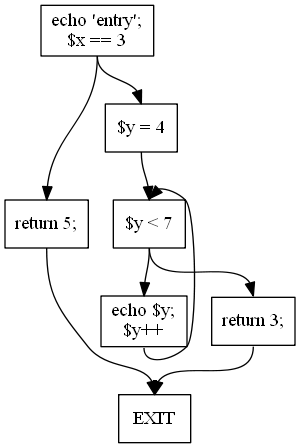
\includegraphics[scale=0.7]{img/cfg.png}
  &
 
\begin{minipage}{6cm}
%pygmentize_begin php
%   echo 'entry';
%   if ($x == 3)
%       $y = 4;
%   else
%       return 5;
%        
%   while ($y < 7) {
%       echo $y;
%       $y++;
%   }
%
%   return 3;
%pygmentize_end
\begin{Verbatim}[commandchars=\\\{\}]
   \PY{k}{echo} \PY{l+s+s1}{\PYZsq{}entry\PYZsq{}}\PY{p}{;}
   \PY{k}{if} \PY{p}{(}\PY{n+nv}{\PYZdl{}x} \PY{o}{==} \PY{l+m+mi}{3}\PY{p}{)}
       \PY{n+nv}{\PYZdl{}y} \PY{o}{=} \PY{l+m+mi}{4}\PY{p}{;}
   \PY{k}{else}
       \PY{k}{return} \PY{l+m+mi}{5}\PY{p}{;}
        
   \PY{k}{while} \PY{p}{(}\PY{n+nv}{\PYZdl{}y} \PY{o}{\PYZlt{}} \PY{l+m+mi}{7}\PY{p}{)} \PY{p}{\PYZob{}}
       \PY{k}{echo} \PY{n+nv}{\PYZdl{}y}\PY{p}{;}
       \PY{n+nv}{\PYZdl{}y}\PY{o}{++}\PY{p}{;}
   \PY{p}{\PYZcb{}}

   \PY{k}{return} \PY{l+m+mi}{3}\PY{p}{;}
\end{Verbatim}
\end{minipage}

  \\
  \end{tabular}
  \caption{Control flow graph\label{cfg}}  
\end{table}        
        
        %---------------------------------------------------------------------------------------
        \subsection{Transfer functions}
        
        We say that the input state of a statement is associated with 
        the \emph{program point before} the statement and the output state 
        is associated with the \emph{program point after} the statement. 
        Our aim is to calculate \emph{data-flow} value for both 
        program points for each statement, denoted $IN(s)$ and $OUT(s)$ for 
        a statement $s$.
        
        \subsubsection*{Single Statement}
        
        We can express the \emph{data-flow} for \emph{program point after} 
        a statement as a function of the \emph{data-flow} of 
        \emph{program point before} the statement, also called \emph{transfer function}. 
        Formally if $f_t$ is a \emph{transfer function}, then $f_t(IN(s))=OUT(s)$.
        Each type of statement will have a different \emph{transfer function} 
        that will reflect the semantics of the statement. 
        
        Example: our analysis tracks type of local variables, so the \emph{data-flow} 
        is a map from variable names to their type. In such setting, a \emph{transfer function} 
        for assignment statement \code{\$a=\$b}, will take the input \emph{data-flow} 
        $flow_{in}$ and will return $flow_{out}$, such that $flow_{out}(x)=flow_{in}(x)$ for 
        every variable name $x$, except for $flow_{out}(\$a)=flow_{in}(\$b)$. In other words, 
        the type of all the variables stays the same, except for \code{\$a} whose type 
        changes to whatever is the type of \code{\$b} is. 
        
        In practice, there is only one \emph{transfer function} for all the assignment 
        statements that is parametrized by the left-hand side and right-hand side of 
        the assignment. And in general, each statement in the programming language has 
        usually its ``meta'' \emph{transfer function} that is parametrized not only 
        by the input \emph{data-flow}, but by the statement structure.
        
        \emph{Transfer functions} are often described in the form of inference rules. 
        An example of an inference rule can be 
        ``if the type of variable \code{b} is \code{Integer} in state $S_1$, 
        then after executing statement \code{a=b}, we get a new state $S_2$ that 
        is the same as $S_2$ except variable \code{a} is of type \code{Integer} in $S_2$''. 
        Those rules can be more formally described with the following notation        
        $$
        \infer{a:Integer\in{}S_2}{b:Integer \in S_1, [a=b, S_1] \rightarrow S_2}
        $$        
        where above the horizontal line we have hypothesis and below is 
        the conclusion. In hypothesis we have that in state $S_1$ it 
        holds that $a$ is an integer and a statement $a=b$ transforms 
        the state $S_1$ to $S_2$. The conclusion says that in state 
        $S_2$ $b$ is an integer. We should also say that other 
        facts in $S_2$ stay the same as in $S_1$, in other words they 
        are not changed by the transformation, but for the sake 
        of brevity, we will always assume that implicitly.
        
        \subsubsection*{Statement Interaction}
        
        The \emph{data-flow} for \emph{program point before} a statement 
        depends on the \emph{data-flow} of \emph{program point after} the 
        last executed statement. Let us consider a basic block $B$ with 
        statements $s_0, s_1, ..., s_n$.
        
        In the case of any $s_i \neq s_0$, that is any statement but 
        the first one, there is only one statement whose execution 
        can precede the execution of $s_i$ and that is the previous statement 
        in the sequence: $s_{i-1}$. So we have $IN(s_i) = OUT(s_{i-1})$ 
        for $i\in{[1..n]}$. 
        
        In fact, thanks to this property, we can define \emph{transfer function} 
        $f_B$ of a basic block as composition of transfer functions of 
        its statements. Formally: 
        
        \[ f_B = f_{s_n} \circ f_{s_{(n-1)}} \circ ... f_{s_0} \]
        
        where $f_{s_i}$ is the transfer function for statement $s_i$.            
        Furthermore, we denote \emph{data-flow values} of basic block as 
        $IN(B)=IN(s_1)$ and $OUT(B)=OUT(s_n)$. From the definitions we can 
        observe simple identities: 
        
        \[ f_B(IN(s_1))=f_B(IN(B))=OUT(B)=OUT(s_n) \]
        
        The first statement $s_1$ of the basic block has to be 
        handled differently. Its execution can be preceded by 
        execution of the last statement of any of 
        the basic blocks $B_1, B_2, ..., B_m$ that precede basic block 
        $B$ in the control flow graph. One of the possibilities to deal with 
        this, is to combine \emph{data-flows} $OUT(B_1), ..., OUT(B_m)$ into 
        single \emph{data-flow} that approximates all of them. 
        Nonetheless, the way the \emph{data-flows} are combined depends 
        on the concrete \emph{data-flow} type and thus 
        should be defined by the analysis. We denote the function to 
        combine \emph{data-flows} as $\mathit{MEET}$. 
        
        \subsubsection*{Equations for Data-Flow}
        
        When we put everything together, we get a set of equations:
        \begin{align*}
            OUT(B_i) &= f_{B_i}(IN(B_i)) \\
            IN(B_i) &= \mathit{MEET}(OUT(P_0), ..., OUT(P_m)) \\ 
        \end{align*}
        where $P_0, ..., P_m$ are predecessors of $B_i$ in the 
        control flow graph. The analysis must also define value 
        of $IN(START)$, that is \emph{input state} for the 
        initial node, which does not have any predecessors.
        
        \subsubsection*{Example}
        We will illustrate the system of \emph{data-flow} equations on a 
        simple example. The subject of our analysis will be the 
        type of the variable \code{\$i} in the code sample in figure \ref{dfacfg}.
        
        \emph{Data-flow} will be a set of possible types of variable $i$ and 
        initial \emph{data-flow} of the start node will be an empty set.

\begin{table}[h]
  \begin{tabular}{ l | m{6cm} }
  \centering
    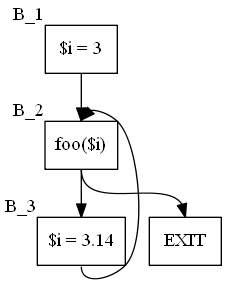
\includegraphics[scale=0.7]{img/dfa-cfg.png}
  &
 
\begin{minipage}{6cm}
%pygmentize_begin php
%   $i = 3;
%   while (foo($i)) {
%       $i = 3.14;
%   }
%   // exit
%pygmentize_end
\begin{Verbatim}[commandchars=\\\{\}]
   \PY{n+nv}{\PYZdl{}i} \PY{o}{=} \PY{l+m+mi}{3}\PY{p}{;}
   \PY{k}{while} \PY{p}{(}\PY{n+nx}{foo}\PY{p}{(}\PY{n+nv}{\PYZdl{}i}\PY{p}{))} \PY{p}{\PYZob{}}
       \PY{n+nv}{\PYZdl{}i} \PY{o}{=} \PY{l+m+mf}{3.14}\PY{p}{;}
   \PY{p}{\PYZcb{}}
   \PY{c+c1}{// exit}
\end{Verbatim}
\end{minipage}

  \\
  \end{tabular}
  \caption{Code for Data-Flow Example\label{dfacfg}}  
\end{table}

        \emph{Transfer functions}: we will assume that a function call does 
        not change state, therefore the transfer function of 
        function call is identity -- $OUT(s)=IN(s)$. Assignment of 
        a constant \code{c} of type \code{T} to \code{\$i} changes 
        type of \code{\$i} to \code{T}.
        
        \emph{MEET} operation will be union of the sets of 
        possible types of \code{\$i}.
        
        The set of equations is in this case
        
        \begin{align*}
            OUT(B_1) &= f_{B_1}(IN(B_1))=f_B(\emptyset) \,\,\,\,\,\text{(initial node)} \\
            OUT(B_2) &= f_{B_2}(\mathit{MEET}(OUT(B_1), OUT(B_3))) \\
            OUT(B_3) &= f_{B_3}(OUT(B_2))     
        \end{align*}
        
        Knowing that $f_{B_1}$ and $f_{B_3}$ are constant functions, because 
        the assignment changes type of \code{\$i} to \code{T} without taking 
        the \emph{input data-flow} into account, and $f_{B_2}$ is identity 
        function, we can simplify the equations to

        \begin{align*}
            OUT(B_1) &= \left\{ \mathit{Integer} \right\} \\
            OUT(B_2) &= f_{B_2}(\mathit{MEET}(OUT(B_1), OUT(B_3))) \\
            OUT(B_3) &= \left\{ \mathit{Double} \right\} \\
            \\
            OUT(B_1) &= \left\{ \mathit{Integer} \right\} \\
            OUT(B_2) &= f_{B_2}( \left\{ \mathit{Integer} \right\} \cup \left\{ \mathit{Double} \right\} ) = 
                \left\{ \mathit{Integer}, \mathit{Double} \right\} \\
            OUT(B_3) &= \left\{ \mathit{Double} \right\}
        \end{align*}
        
        With this result we can, for example, check that function \code{foo} 
        is invoked with correct argument type, because from $IN(B_2)$ we 
        know that \code{\$i} at the moment of invocation of \code{foo} 
        can be either of type \code{Integer} or \code{Double}.
                
        \subsection{Finding Solution for the Data-flow Equations}
        
        \subsubsection*{Lattices.}
        The algorithm for finding a solution to a set of data-flow 
        equations is based on algebraic structures called lattices. 
        A lattice is a partially ordered set in which every 
        two elements have a least upper bound, called supremum, 
        and a greatest lower bound, called infimum. If $a$ and 
        $b$ are elements of a lattice, we denote their least upper 
        bound as $a\wedge{}b$.
        
        \emph{Bounded lattice} is a lattice that has 
        a greatest element and a least element, 
        usually denoted as $\top$ and $\bot$. 
        A bounded lattice is depicted in figure \ref{lattice}.       
        
\begin{figure}[h]  
  \centering
    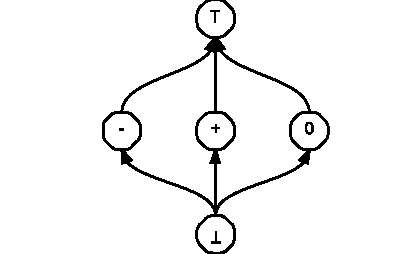
\includegraphics{img/lattice.pdf}
  \caption{Bounded lattice with 5 elements.\label{lattice}}    
\end{figure}

        There are several properties of lattices important for DFA.
        
        If we have a finite bounded lattice $(S, \leq_{s})$ and a function 
        $f:S\rightarrow{S}$ that is monotonous, in order words, 
        $\forall{a,b\in{S}}: a\leq_s{b} \Rightarrow f(a)\leq_s{f(b)}$, 
        then $\forall{x\in{S}}$ $\exists{k\in\mathbb{N}}$, such that 
        $f^k(x)=f^{(k+1)}(x)$. $f^k(x)$ is called a fixpoint.
        
        Intuitively, $f$ has to have a fixpoint because 
        for every argument $y$, it must either return 
        $y$ itself, but then $y$ is a fixpoint, or it 
        returns another element that is strictly 
        greater than $y$, but this cannot go on forever, because eventually 
        $f$ will be given $\top$ for which it does not have 
        any other option but returning $\top$ and we 
        have a fixpoint again.
        
        From this property further follows that if we use a finite 
        lattice's elements as a domain for transfer functions, 
        and the transfer functions are monotonous, then the set of 
        data-flow equations has a solution, which is a safe 
        approximation of the, in a sense, best solution to the 
        data flow problem. Details can be found in \cite{kildall1973unified}.
        
        Product lattice obtained from two or more lattices 
        is also a lattice, which can simplify the design of 
        data flow analyses.

        Power set $\mathcal{P}(S)$, the set of all subsets of $S$, 
        is also a lattice, the lattice order relation 
        being subset relation $\subseteq$.

        \subsubsection*{The Iterative Algorithm}
        
        The algorithm to find the solution to the data-flow equations 
        initially sets $OUT(B_i)$ for every basic block to the initial 
        \emph{data-flow}, which should be the lowest element of the lattice. 
        Then it iteratively takes a basic block $B_j$ such that 
        its input \emph{data-flow} $IN(B_j)$ has changed or is not 
        initialized yet and computes $OUT(B_j)$, which might change 
        the input \emph{data-flow} of the ancestors of $B_j$. 
        The process is repeated until a the system stabilizes. 
        
        The algorithm can take basic blocks in any order, however, 
        the \emph{reverse post order} provides the best time complexity 
        \cite{aho1985compilers}.
        
        \subsubsection*{Bit Vectors as Data-flow Representation}

        The performance of the algorithm also depends on the implementation 
        of \emph{data-flow}, the $\textit{MEET}$ operations and the transfer 
        functions. 
        
        \emph{Data-flow} often represents a subset of a set of possible values 
        and the $\textit{MEET}$ operation is either union or intersection.
        For example, a subset of all possible types of a variable. 
        Furthermore, we want to calculate the information for all 
        variables not only for one. If we know the number of variables $n$ and 
        types $m$ in advance, we can represent the \emph{data-flow} as 
        a bit-vector where groups of $m$ bits represent a data of 
        single variable and within those bits, value of bit with 
        index $i$ indicates whether the type with index $i$ is in the set. 
        Union or intersection can be implemented using fast bitwise operations.


        % -----------------------------------------------------------------------
        \subsection{Abstraction}
        
        The \emph{data-flow} value for program point is typically an abstraction 
        of some property of the set of all possible program states that can be 
        observed during real execution for that program point. 
        
        Abstracting the desired property is often important in order to make 
        the analysis practical or even feasible. Let us consider an analysis 
        that should determine the sign of integral variables at each program point.
        We can have inference rules of the following form.
        
        $$
        \infer{[v_3=v_1+v_2, S_1] \rightarrow S_2, S_2 \vdash v_3 : -7 (sign: \ominus)}
        {S_1 \vdash v_1 : -10 (sign: \ominus) & S_1 \vdash v_2 : 3 (sign: \oplus)}
        $$
        
        However, the implementation would not be very efficient and also the full 
        information about variables values is not always available, but in some cases 
        we can deduce another less precise, but still useful piece of information 
        by other means. For example, variable of type \code{unsigned integer} will 
        always be positive, we can count on that even if we do not know the actual value. 
        What we can do is to abstract the possible integral values with set 
        $\{0, \ominus, \oplus\}$ with the following meanings         
        \begin{itemize}
            \item $\ominus$ represents all negative integers,
            \item $\oplus$ represents all positive integers,
            \item $0$ represents zero,
        \end{itemize}                
        and rewrite the inference rules as follows:
        
        $$
        \infer{[v_3=v_1+v_2, S_1] \rightarrow S_2, S_2 \vdash v_3 : \ominus}
        {S_1 \vdash v_1 : \ominus & S_1 \vdash v_2 : \ominus}
        $$
        
        Nonetheless, there is another problem. What to do when we have $\ominus$ 
        and $\oplus$ in the hypothesis.
        
        $$
        \infer{[v_3=v_1+v_2, S_1] \rightarrow S_2, S_2 \vdash v_3 : ?}
        {S_1 \vdash v_1 : \ominus & S_1 \vdash v_2 : \oplus}
        $$
        
        The solution is to extend the domain so that it is closed under all operations. 
        We add another element to our set:
        \begin{itemize}
            \item $\top$ represents an unknown value (either positive, negative, or zero).
        \end{itemize}
        Then the rule will be:
        
        $$
        \infer{[v_3=v_1+v_2, S_1] \rightarrow S_2, S_2 \vdash v_3 : \top}
        {S_1 \vdash v_1 : \ominus & S_1 \vdash v_2 : \oplus}
        $$        
        
        And for example another rule dealing with $\top$ in hypothesis:
        $$
        \infer{[v_3=v_1+v_2, S_1] \rightarrow S_2, S_2 \vdash v_3 : \top}
        {S_1 \vdash v_1 : \ominus & S_1 \vdash v_2 : \top}
        $$
        
        It is no surprise that we used symbol $\top$, which is also used to denote the 
        greatest element in a lattice. By adding $\bot$, the least element, and inference 
        rules for it, we can get a lattice depicted in \ref{lattice} and use 
        this abstraction as \emph{data-flow} value.
        
        \subsubsection*{Formalization}

        There is a theoretical framework for designing sound and correct 
        abstractions. In a nutshell, an abstraction following this framework 
        has to include: 
        
        \begin{itemize*}
            \item concrete domain $C$, which has to be a lattice ,
            \item abstract domain $A$, which has to be a finite lattice,
            \item concretization function $\gamma{}:A\mapsto{}C$,
            \item abstraction function $\alpha{}:C\mapsto{}A$,
        \end{itemize*}
        
        In our case the concrete domain could be the power set of all 
        possible integral values, which is a lattice, and the abstract 
        domain with elements $\{0, \ominus, \oplus\, \top, \bot\}$ was 
        described above. The $\gamma$ and $\alpha$ functions map values 
        from one domain to another. When we map elements of concrete domain 
        to the abstract domain, we loose precision due to abstraction. 
        Let us provide few examples, instead of a formal definition 
        of $\gamma$ and $\alpha$.
        
        \begin{align*}
            \begin{split}
                \gamma{}(\oplus) &= \left\{1, 2, 3, ...\right\} \\
                \gamma{}(\top) &= \top = \left\{..., -2, 1, 0, 1, 2, ...\right\} \\
            \end{split}
            \begin{split}
                \alpha{}(\left\{3, 4, 5\right\}) &= \oplus \\ 
                \alpha{}(\left\{3, -4\right\}) &= \top \\
            \end{split}
        \end{align*}
        
        The framework for abstract interpretation further defines 
        necessary conditions for the $\gamma$ and $\alpha$ functions 
        and conditions for the \emph{transfer functions} with respect 
        to $\gamma$ and $\alpha$ mapping. Details and other 
        static analysis methods based on abstract interpretation 
        framework can be found in \cite{cousot1977abstract}, 
        \cite{Cousot2000abstract}.

        % ----------------------------------------------------------------------
        \subsection{Intraprocedural Analysis}
        
        So far we have been discussing an analysis of a single function 
        or a method \footnote{We will use term 
        routine to designate a global function, static or instance method}. 
        However, if we want to analyse a whole program or 
        a library, the interaction between the routines 
        must be taken into account.
        
        A straight forward approach is to regard other routines as 
        black boxes and assume the worst with respect to how a 
        routine call can change the program state. Nonetheless, 
        in practical programming language with references, or pointers,  
        pass-by-reference arguments, lambda functions with 
        capture by reference, and other caveats, an innocent 
        routine call can theoretically do almost anything to 
        the program state even from the local point of view 
        of the function we are analysing.
                
        \subsubsection*{Context Sensitive Intraprocedural Analysis}
        
        The most precise solution is to analyse a function, 
        say \code{foo}, for each possible calling context. 
        In other words, re-analyse \code{foo}'s body every 
        time we encounter its invocation when analysing another 
        function, and use the program state before 
        the invocation of \code{foo} as an initial state 
        for the re-analysis of \code{foo}.
        
        Caching of the results of analysis based on 
        the calling context, so that we do not re-analyse it 
        if the context is the same as some context previously 
        encountered, is possible. However, in the most generic 
        form, it is impossible to asses the equality of 
        program states, because the context consists not only 
        of arguments passed to the function, but also the 
        global state including the heap.
        
        Another problem, which makes fully context sensitive 
        approach impractical or even impossible, is polymorphism 
        or dynamic invocation of routines in general, be it 
        lambda functions, virtual methods, reflection, 
        or any other means. It is not known statically what 
        function will be invoked and thus what function to analyse. 
        The call site can be determined by the analysis itself, 
        but in general it cannot be guaranteed.
        
        \subsubsection*{Heap Abstractions}
        
        When a routine takes a pointer or reference to some object 
        on the heap as an argument, it can traverse to other 
        objects on the heap and change their state. Let alone low-level 
        languages that allow direct manipulation with the memory and 
        can therefore change anything in the heap. 
        
        The heap can be important part of the program state for 
        some kinds of analyses. If we want to take the heap state 
        into the consideration during the analysis, we need an 
        abstraction for the heap to make the approach feasible 
        in practice.
        
        Researchers have proposed several approaches to representation 
        of heap data in an abstract way to minimize memory requirements 
        and provide fast algorithms to check two heap abstractions 
        for equality or isomorphism. A sound and useful definition 
        of heaps isomorphism is also a problematic task by itself. 
        The paper \cite{kanvar2014heap} provides a survey on the heap 
        abstraction models.
        
        \subsubsection*{Region Based Analysis}
        
        Another approach is to analyse a routine once in a 
        generic context setting and create a \emph{transfer function} 
        that summarizes the effects of the routine call to the 
        program state \cite{aho1985compilers}. However, in practical setting, 
        we need to decide how to derive the \emph{transfer function} and how to 
        represent it. A constant \emph{transfer function} that always 
        returns the $\top$, in other words, the worst assumption about 
        the program state, is always safe \emph{transfer function} 
        for any routine call, but we have not gained anything over 
        the naive solution from the beginning of this section.
        
        In the case of Control Flow for Phalanger, we used 
        a variant of a region based analysis. Details are 
        discussed in the following \wsection{}.
    
    % ----------------------------------------------------------------------------
    \section{Control Flow for Phalanger Approach}
        
        \subsection{Assumptions}        
        The approach taken in Control Flow for Phalanger is based on an 
        observation that even when developers are given a dynamically typed 
        programming language, it does not mean that they will write 
        dynamically typed programs. Empirical evidence for this 
        observation was presented in \cite{walker1996type}. 
        
        We are therefore assuming that large part of the analysed 
        code corresponds to a statically typed code one-to-one, 
        it only does not include the type information. However, 
        we do not want to ignore the dynamic typing completely.

        Another decision we made, is that only local variables 
        will be a viable target for compiler optimizations use 
        case, since the compiler optimizations have to be safe with 
        respect to all the possible and obscure corner cases, 
        and global variables and heap memory are difficult to 
        analyse precisely. On the other hand, with bug-hunting and 
        integrated development environment supporting style 
        analyses, we can afford more courageous assumptions.
        
        In this \wsection{} we focus on the type analysis, because 
        it is by far the most complex kind of analysis implemented. 
        Other analyses, like constant propagation, follow the same 
        concepts and, furthermore, they rely on the results of the 
        type analysis and points-to analysis, which is 
        also discussed in this \wsection{}.
        
        \subsection{Analysis Results}
        
        The outcomes of the analysis of a single routine are:
        
        \begin{description*}
            \item[Variables table: type information for local variables] -- 
            for every local variable, a set of its possible types at any 
            point during the execution of the routine. Note that it summarizes 
            all types that variable can have at different program points. 
            Knowing that a variable has only one possible type can be useful 
            for compiler.
            
            \item[Type information for expressions] -- every expression in the 
            routine's body will be annotated with the type or set of types 
            the expression can evaluate to.
            
            \item[Warnings] -- some expressions expect only operands of 
            certain type; if the analysis encounters such expression 
            and from the analysis it follows that the operand is not of the 
            expected type, the piece of code in question is reported as a warning.
            The same holds for the type expectations extracted from 
            documentation comments for fields, routines and others.
            
        \end{description*}
        
        Another outcome of analysis across all routines will be \emph{globals table} 
        with type information for global symbols that is global variables, 
        instance and static fields and routines.
        
        \subsection{Local Analysis: Overview}
        
        We can think about expressions in terms of 
        evaluation trees, like in figure \ref{evaltree}. 
        Since expressions should be annotated with their 
        type information, the analysis can use a bottom 
        up approach and annotate the leaves of the 
        evaluation tree first and then recursively from 
        the type information of operands infer type 
        information for compound expressions.
        
        \begin{figure}[h]  
          \centering        
          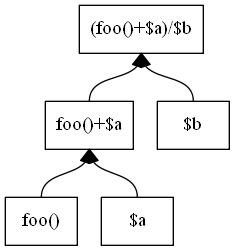
\includegraphics[scale=0.5]{graphs/evaltree.png}
          \caption{Evaluation tree of an expression \code{(foo()+\$a)/\$b}.\label{evaltree}}    
        \end{figure}        
        
        Statements or expressions that can change the program state, 
        like assignment statement, will have their operands 
        annotated with the type information and thus have all 
        the necessary information to reflect the change of 
        the program state accordingly. For instance, 
        the type of the right hand side expression of an assignment 
        statement will determine the new type for the variable 
        on the left hand side.
        
        Some type information can be inferred from the code without 
        any knowledge about variables' types. For example, the result 
        of string concatenation is always a \code{string}, no matter 
        what the types of the arguments are. However, simple local 
        variable use is an expression and we need to know the possible 
        types of the variable to annotate this expression 
        with its type. For this, we need to perform a DFA that will 
        give us the type information for each variable at each program 
        point. Note that the \emph{data-flow} values are used only 
        temporarily to annotate the expressions and build the variables 
        table, but we do not create actual \emph{data-flow} instance 
        for every program point.
        
        The questions that have to be answered, in order to 
        implement the DFA, include:
        
        \begin{itemize*}
            \item what the \emph{data-flow} values will be, 
            \item what data structures will be used to represent them efficiently, 
            \item how to deal with routines calls and their effects to the program state.
        \end{itemize*}
        
        \subsection{Local Analysis: Data-flow Values}
        
        The \emph{data-flow} should capture the type information 
        for variables within the routine. We do want to support 
        dynamic typing, therefore for every variable, we have 
        a subset of all its possible types, not only a single type.        
        The \emph{data-flow} value is a map from variable names to 
        subsets of types. 
        
        For an efficient representation of the \emph{data-flow}, 
        the routine's body is scanned for all local variables names 
        referenced types prior to the analysis. After the scan, the 
        number of variables and types is a known constant and the 
        \emph{data-flow}, being an array of subsets of a set 
        of all the types, can be represented as a bit-vector. 
        The $\operatorname{MEET}$ operation is a union, because if 
        a variable can have type \code{T} from one branch and 
        type \code{K} from another, at the join point we can only 
        assume that it has either type \code{T} or \code{K}.
        
        However, with a real world class based object oriented 
        programming language, the situation is not as simple. 
        We have to deal with subtyping, and we also want to 
        support type information from documentation comments, 
        which nonetheless should be distinguished from the 
        type information inferred from the actual code.
        
        The basic \emph{data-flow} values for a single variable 
        and set of types $\left\{int, false, null\right\}$ are depicted 
        in the figure \ref{typeslattice1}. Aside the whole set of 
        all types references within the routine's body, we have 
        another artificial value called \emph{Any}, which simply 
        designates any possible type, not restricted to the set 
        of known types. In the following paragraphs, we discuss 
        how we added support for classes and documentation 
        comments to this schema. We focus on \emph{data-flow} 
        lattice for a single variable; the lattice for all variables 
        will simply be a product lattice.
        
        \begin{figure}[h]  
          \centering        
          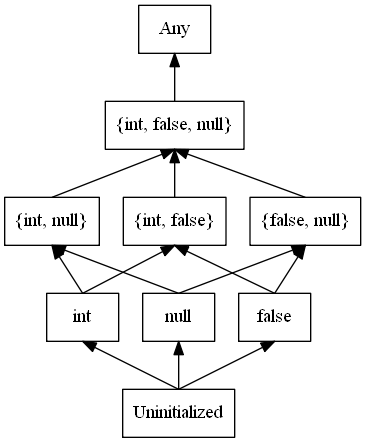
\includegraphics[scale=0.6]{graphs/types-lattice1.png}
          \caption{Basic lattice with types.\label{typeslattice1}}    
        \end{figure}
        
        \subsubsection*{Booleans}        
        In the case of booleans, we distinguish 
        \code{true} and \code{false}, because it is a well 
        known pattern in PHP for routines to use \code{false} 
        return value as an indication of failure. 
        Routines then can have, for example, have type 
        \code{false|object} meaning that this routine returns either 
        object or value \code{false}, never value \code{true}.
        
        \subsubsection*{Null}        
        Another thing to note is that we treat \code{null} as 
        a special type. This again comes from PHPDoc documentation 
        comments, where one can, for instance, state 
        \code{integer|null} as return type of a routine, 
        in which case representing the routines return type 
        as just \code{integer} would not be precise. Moreover, 
        having \code{null} can be used to distinguish between 
        non-nullable and nullable reference types. 
        Control Flow for Phalanger by default assumes that all 
        the reference types can be \code{null}, but it can 
        be configured to assume the opposite, in which case it can, 
        for example, report type error if a routine expects 
        instance of some \code{object} as an argument, 
        but is given \code{null}.
        
        \subsubsection*{Type Hints}        
        We refer to the type information gathered from documentation 
        comments as type hints. For example, routines can have 
        documentation comments that state expected types of the 
        parameters. However, it is perfectly legal to invoke the 
        routine with actual parameters of different types, so we 
        cannot rely on the documentation completely, but we want 
        to utilize it.
        
        For this purpose, we distinguish between type information 
        that was inferred from the code and should always be 
        valid and type information that was extracted from the 
        documentation comments or possibly other unreliable 
        sources, for instance, return type of a non-final method, 
        which cannot be accurately determined because of 
        polymorphism.
        
        The distinction is realized as a single bit flag 
        we call ``type hint''. It is a single flag for the 
        whole set of possible types, so we cannot have a 
        set of two possible types where one is ``type hint'' 
        and the other is not. 
        
        We can think of all the sets with ``type hint'' flag 
        as a parallel lattice to the lattice of sets without 
        ``type hint'' flag. Let us say that $hint(x)$ denotes 
        an element from the parallel lattice corresponding to 
        element $x$ in the original one. If we are comparing 
        two elements $a$ and $b'$, where $b'=hint(b)$ is from the 
        ``type hint'' lattice, we say that their upper bound or 
        supremum is equal to $hint(a\wedge{}b)$, formally 
        $a\wedge{}b'=hint(a\wedge{}b)$. A lattice that is formed 
        from putting together the original types lattice and the 
        ``type hint'' lattice for types $\left\{int, string\right\}$ 
        is depicted in figure \ref{hintslattice}.
        
        \begin{figure}[h]  
          \centering        
          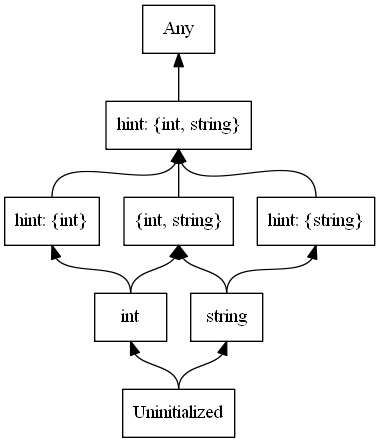
\includegraphics[scale=0.6]{graphs/hints-lattice.png}
          \caption{Types lattice with ``type hint'' flag.\label{hintslattice}}    
        \end{figure}
        
        
        \subsubsection*{Classes}
        
        We refer to built-in types as basic types, those are 
        \begin{multicols}{2}
        \begin{itemize*}
            \item int
            \item double
            \item string
            \item resource
            \item false and true (instead of boolean)
            \item null
            \item array
            \item callable -- for example: lambda
        \end{itemize*}
        \end{multicols}
        
        If we say that variable \code{\$a} is of type \code{T}, 
        where \code{T} is a non-final class, even in statically 
        typed language, this could mean that \code{\$a} can 
        be in fact instance of many different classes, 
        namely \code{T} and all its subclasses.
        
        Because we are in a dynamic environment, we cannot, 
        in general, know all subclasses of \code{T} in advance. 
        Nonetheless, it can be useful to distinguish between 
        ``\code{\$a} is of type \code{T} only'' and 
        ``\code{\$a} is of type \code{T} or any of its subtypes''.
        
        To make this distinction, we add another flag ``subclasses'', 
        which works similarly to ``any type'' flag: it holds or does 
        not hold for the whole set of class types. Also the upper bound 
        of two elements, where one of the has the flag ``subclasses'', 
        will has the ``subclasses'' flag.
        
        Moreover, we add one artificial value, which is \code{object}, 
        and it denotes arbitrary class instance, but it is not the 
        same as \emph{Any}, because it excludes the other primitive 
        types. A lattice for just class types $\left\{T,K\right\}$ 
        is in figure \ref{objectslattice}.
        
        \begin{figure}[h]  
          \centering        
          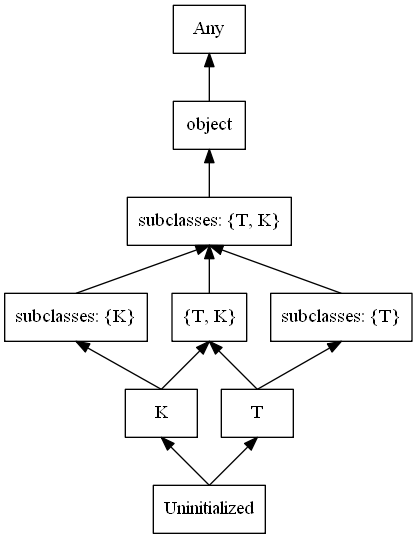
\includegraphics[scale=0.5]{graphs/objects.png}
          \caption{Types lattice with classes.\label{objectslattice}}    
        \end{figure}        
        
        The upper bound of any set of class types and a set of 
        basic types is a union of those. However, the upper 
        bound of a set with some class types in it and a set with 
        \code{object} in it is a union of the basic types and 
        \code{object}, so the class types are ``overridden'' by 
        the \code{object}. This is illustrated in figure \ref{objectsandbasics}.
        
        \begin{figure}[h]  
          \centering        
          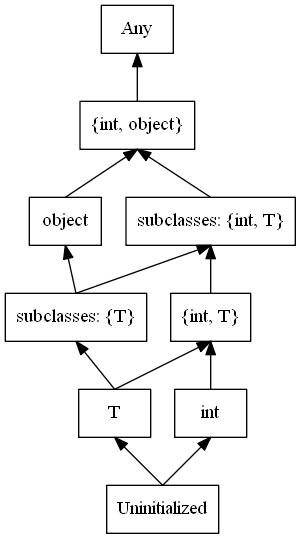
\includegraphics[scale=0.5]{graphs/objects-prim.png}
          \caption{Types lattice: class and a basic type.\label{objectsandbasics}}    
        \end{figure}
        
        This lattice with class types can be amended with the ``type hint'' 
        flag the same way we did before we introduced classes.
        
        \subsection{Intraprocedural Analysis}
        
        The approach we described so far considers only local variables, 
        but we want to analyse object and class fields' types, and global 
        variables. We also have to take into account possible changes to 
        local variables made from other routines through references.
        
        The assumption here is that the results of analysis for fields 
        and global variables do not have to be precise and that although 
        PHP is a dynamic language that permits dynamic fields and dynamic 
        methods, mostly the developers do not abuse those features and 
        we can assume that instances of the same class have the same 
        fields of the same type and the same methods across the whole 
        program. Furthermore, routines return type and expected 
        arguments types will mostly be constant and independent 
        from the program state or each other.
        
        \subsubsection*{Routines Return Values}
        When the analysis encounters a routine invocation, it needs 
        to know the routine's return type and possible other pieces 
        of information we discuss later.
        
        If the source code of the routine in question is available, 
        in other words, it is part of the analysed source, we 
        recursively trigger its analysis in order to infer its 
        return type. When the analysis finished, we save the 
        results to the \emph{globas table} so that we do not 
        need to analyse the routine next time and resume the 
        analysis of the original routine.
        
        This approach, however, does not work for recursive 
        and mutually recursive routines. The solution we use 
        is that if a cycle in routines invocations is detected, 
        we do not analyse the last routine in the cycle, but 
        instead we assume the worst about its return type -- 
        we assume it can return any type.
        
        
        \subsubsection*{Heap}        
        Let us first provide an example, where heap abstraction and 
        context sensitive intraprocedural analysis would be useful:
        
%pygmentize_begin php
% function foo() {
%   $a = new X();
%   boo($a);
%   return $a->bar;
% }
%
% function boo(X $a) {
%   $a->bar = 3;
% }
%pygmentize_end
\begin{Verbatim}[commandchars=\\\{\}]
 \PY{k}{function} \PY{n+nf}{foo}\PY{p}{()} \PY{p}{\PYZob{}}
   \PY{n+nv}{\PYZdl{}a} \PY{o}{=} \PY{k}{new} \PY{n+nx}{X}\PY{p}{();}
   \PY{n+nx}{boo}\PY{p}{(}\PY{n+nv}{\PYZdl{}a}\PY{p}{);}
   \PY{k}{return} \PY{n+nv}{\PYZdl{}a}\PY{o}{\PYZhy{}\PYZgt{}}\PY{n+na}{bar}\PY{p}{;}
 \PY{p}{\PYZcb{}}

 \PY{k}{function} \PY{n+nf}{boo}\PY{p}{(}\PY{n+nx}{X} \PY{n+nv}{\PYZdl{}a}\PY{p}{)} \PY{p}{\PYZob{}}
   \PY{n+nv}{\PYZdl{}a}\PY{o}{\PYZhy{}\PYZgt{}}\PY{n+na}{bar} \PY{o}{=} \PY{l+m+mi}{3}\PY{p}{;}
 \PY{p}{\PYZcb{}}
\end{Verbatim}
        
        Here the function \code{boo} changes type of the nested field 
        \code{bar}. If we do not reflect this in the program 
        state after the invocation of \code{boo(\$a)} in 
        function \code{foo}, we cannot determine the type of 
        the return expression \code{\$a->bar}.
        
        However, we decided to approach this problem differently. 
        We do not analyse individual object instances, 
        instead we summarize the type information inferred 
        for individual instances of the same class and provide 
        those results within the \emph{globals table}.
        
        Illustrated on the same example, when analysing function 
        \code{foo}, the analysis would encounter the invocation 
        of \code{boo}. Since \code{boo} has not been analysed yet, 
        this triggers analysis of \code{boo}. While analysing 
        \code{boo} the \emph{globals table} learns that 
        field \code{bar} can be of type \code{integer}. When analysis 
        of \code{boo} finishes and analysis of \code{foo} resumes, 
        on the line with \code{return \$a->bar} we know from the 
        \emph{data-flow} that \code{\$a} is of type \code{X} and 
        from the \emph{globals table} we get that field \code{bar} 
        of class \code{X} can be of type \code{integer}.
        
        With this approach we do not have to model heap, 
        which can be more effective, but on the other hand, 
        there are cases different to this example, where our 
        approach fails to devise any useful information 
        and heap model, could give us 
        better results. For instance, if function \code{boo} 
        did not provide type information for its parameter 
        in its signature, because we analyse each routine 
        in a generic context.
                
        Moreover, we ignore the effects of indirect assignments 
        and references to the \emph{globals table}, which means 
        that the \emph{globals table} is not safe approximation. 
        However, as we stated at the beginning of this \wsection{}, 
        the analysis of instance fields is meant for bug hunting 
        purposes and we can afford some imprecision. In addition, 
        the type information inferred by means of \emph{globals table} 
        is marked with the ``type hint'' flag.
        
        The global variables and static class field are analysed 
        in the way as instance fields.
        
        \subsubsection*{Type Documentation}
        There are two different cases where we need to consider type 
        information for fields or global variables: when a field or global 
        variable is read, and when a field or global variable is assigned to.
        
        Field and global variables can have PHPDoc type documentation.
        In the case of assignment, we want to check that the value assigned 
        to the variable has a type compatible with the documentation, 
        otherwise it is possibly a bug or documentation error.
        
        When it comes to type annotation of an expression that uses 
        a global variable or a field, if the type documentation is available, 
        we use it over the information from \emph{globals table}, 
        but still mark the type information with ``type hint'' flag.
        
        \subsubsection*{References Analysis}
        References in PHP are used, but occasionally, therefore we do 
        not want to ignore them, but we do not require a 
        precise results when references are used in 
        the analysed routine.
        
        Another piece of information the analysis needs to know 
        about a routine that is being invoked from within the 
        analysed routine is which arguments are passed by reference 
        to it, so that their value can be changed inside the 
        invoked function. This is fortunately a part of the 
        routine's signature, and can be easily determined. 
        We simply throw away any assumptions we had about the type 
        of a variable which is being passed by reference to 
        another routine.
        
        The situation is more complicated with references within a 
        single routine. When a statement or expression can change 
        the type of a variable, it can change type of any variable 
        that this variable points to, if it is a reference.
        
        We use a simple approach: prior to the analysis, the routine 
        body is scanned for any assignments by reference (\code{\$a=\&\$b}) 
        and two sets are created: variables that can be a reference and 
        variables that can be pointed to by a reference. This is very 
        conservative approximation, but we expect sparse usage of 
        references.
        
        When the analysis finds out that a type of a variable can 
        be changed to \code{T}, it checks if the variable can be 
        a reference and if so the types of all the variables that 
        can be pointed to by any reference are updated. Those variables 
        \textbf{may} only be pointed to, but do not \textbf{have to} 
        be pointed to, so we take their current type information 
        and merge with type \code{T}, creating over approximation.
        
        Moreover, any routine's invocation can change any local 
        variable from the can be pointed to set, because 
        references can ``leak'' on the heap, for where 
        the other routine can read them. That is why, after any routine 
        invocation, we throw away any assumptions about variables 
        in the can be pointed to set.
        
        The same holds for local variables that are captured by 
        reference by some lambda function. The lambda function can 
        again ``leak'' on the heap, from where the other routine 
        can invoke it.
        
        %TODO: \subsubsection*{Arrays}
        
        

\chapter{Related Work}

    A brief overview of the static analysis methods was presented 
    in the previous \wchapter{}. In this \wchapter{}, we focus on 
    tools that also use static analysis to analyse PHP code for 
    different purposes. We also shortly mention interesting tools 
    for other dynamic languages.

    \section{Security Vulnerabilities in Web Applications}
    
    Most of the existing work on static analysis of PHP is 
    focused on discovery of security vulnerabilities in 
    web applications that typically come from improperly 
    handled user input, also called taint-style vulnerabilities. 
    It is important for such analyses to be able to follow 
    the flow of data from global variables like \code{\$\_POST} 
    that contain user input, therefore more precise model of 
    heap memory is required so that flow of data in between 
    object instances and routine calls can be analysed. 
    
    An analysis for security vulnerabilities has also a different 
    model of usage. Such analysis can be run less frequently, 
    for example, only before release or as a part of a continuous 
    build process. Interactive on-the-fly analysis in an 
    integrated development environment could also be a viable 
    use case, but typically not the main goal. Moreover, 
    such analysis is not likely to be run every time the 
    application is to be compiled or interpreted.
    
    Some of the available tools for detecting taint-style 
    vulnerabilities in PHP are Pixy\cite{jovanovic2006pixy} 
    and recently released Weverca: Web Verification Tool\cite{hauzarhunting}.
    
    \subsection{Weverca: Web Verification Tool}
    
    Weverca is an implementation of static analysis framework also 
    based on the Phalanger parser. As opposed to Control Flow for 
    Phalanger, the main goal of Weverca is to provide security 
    vulnerabilities analysis, although it is capable of supporting 
    other kinds of static analyses.
    
    \subsubsection*{Memory Abstraction}
    Weverca represents the program state at each program point by 
    an abstraction of the complete memory state including local 
    variables, global variables and static fields. Compared 
    to our approach, we represent the program state by the state 
    of local variables only and global variables and fields not 
    analysed precisely in context sensitive way, but summarized 
    in one global database shared among all analysed functions.
    
    The approach of Weverca enables better precision and 
    their default implementations of the memory model do 
    provide such precision. On the contrary, our approach 
    permits more effective representation of the program 
    points state. Needless to say, both tools provide means 
    to be extended with an implementation of the other 
    approach.
        
    Moreover, the memory abstraction used in Weverca includes 
    defined symbols, such as routines, classes and others. 
    PHP permits to define symbols dynamically and in certain circumstances 
    symbol cannot be used before it is defined\footnote{A symbol 
    cannot be used before the file with its declaration is imported, 
    but symbols from the same file can be used before they are declared.}. 
    Therefore Weverca is capable of discovering use before 
    declaration kind of errors for global symbols. In Control 
    Flow for Phalanger, we decided to not support this, 
    because most of the modern object oriented PHP projects 
    use \emph{autoloading} and with 
    autoloading it is impossible in general to analyse which 
    files are being imported at which program points. 
    Autoloading rules are often simple and follow 
    similar patterns and so a viable possibility for a static 
    analyser would be to let the user choose from predefined 
    set of autoloading rules that the analyser understands. 
    However, neither of the tools implement this feature yet.
    
    \subsubsection*{Intraprocedural Analysis}
    
    In order to make the interprocedural analysis context 
    sensitive, Weverca inlines the control flow graph of 
    invoked routine in the control flow graph of the 
    analysed routine. Note that there can be more than 
    one routine that can be invoked due to polymorphism 
    or dynamic nature of PHP. In such case Weverca 
    inlines all of them adding a non-deterministic choice 
    between them, in other words, edges from the routine call 
    program point to the first program point of all the 
    possible routines.
    
    As discussed in the previous \wchapter{}, Control Flow for 
    Phalanger uses modular approach, which may scale better, 
    but lacks the precision of Weverca.
    
    \subsubsection*{Type Information}
    
    \note{Support for type hints. Enough for whole subsubsection?}
    
    \subsubsection*{Design and Implementation}
    
    From the point of view of implementation, Weverca uses 
    Phalanger as a parser, but the design does not evince 
    any intention of tighter integration with Phalanger. 
    The version of Phalanger used is slightly outdated, 
    and thereof support for newer PHP language constructs 
    is probably missing.
    
    \note{PHPDoc support.}
    
    \note{Intermediate Representation}
    

    \section{Type Inference}
    
    Type inference for dynamic languages is typically implemented 
    for the purposes of compilation or interpretation. A notable implementation 
    is type inference for PHP in Facebook's Hip Hop project \cite{zhao2012hiphop}, 
    which is a compiler from PHP to C++ and a custom intermediate language 
    that can be run in the Hip Hop virtual machine. Hip Hop performs type 
    analysis in order to find a single type for a variable, so it can treat 
    it as statically typed variable during compilation. However, if a single 
    type for a variable cannot be determined, Hip Hop does not analyse 
    the type information any further and fall backs to the dynamic typing.    
        
    There are implementations of type inference for other dynamic languages. 
    Ecstatic\cite{madsen2007ecstatic} is type inference for Ruby 
    implemented using control flow insensitive cartesian product algorithm. 
    Rubydust\cite{an2011dynamic} introduces a \emph{constraint based dynamic 
    type inference} that infers static types based on dynamic program 
    executions.

    \subsection{Phantm}
    
    Phantm\cite{kneuss2010phantm} is a tool for detection of type related 
    errors. From all the projects mentioned in this chapter, the aim of 
    Phantm is closest to our project, which is why we also used Phantm 
    for evaluation and compared its results with ours in 
    section \ref{phantmresults} Comparison to Phantm.
    
    Phantm uses semi-dynamic and semi-static analysis approach. The web 
    application in question is run up to a defined point, which is invocation 
    of special Phantm's function that collects data about the state of the application, 
    especially, values of global variables. This data is then used as an initial 
    state for static analysis. The dynamic part of the analysis is called bootstrapping. 
    This design illustrates that although type related errors can be searched for 
    in generic frameworks, libraries or, for example, command line utilities 
    written in PHP, Phantm's focus is on complete web applications.
    
    \note{
    \begin{itemize*}
        \item similar type abstraction (null, false, true, int values are repr. explicitly for const. prop.)
        \item heap abstraction, but assumption about routines only changing a 
        local region in heap and returning fresh instances.
        \item array support: merging, termination -- limited nesting.
        \item ignores completely:
            \begin{itemize*}
                \item references
                \item indirect accessed (variables, fields)
                \item assignment in conditional exprs.
                \item eval, autoload
            \end{itemize*}
    \end{itemize*}    
    }

\chapter{Implementation}

    \section{Implementation Specific Constraints}
    
    One of the requirements was that the project should be implemented 
    in the context of the Phalanger project. It should be ready 
    to be plugged in between the Phalanger's front-end and back-end and 
    it should also provide public interface useful for the 
    Phalanger PHP Visual Studio tools.
    
    \subsubsection*{Abstract Syntax Tree}     
    Phalanger front-end parses PHP code 
    into an Abstract Syntax Tree (AST) \cite{aho1985compilers} structure. 
    This structure is then traversed by the back-end using the 
    visitor design pattern \cite{gamma1994design}. Phalanger does not 
    use any other intermediate representation than AST and the 
    back end transforms the AST directly to Microsoft Intermediate Language (MSIL).
    
    In order to reduce the memory consumption and provide better 
    modularity, Phalanger code went through minor architecture 
    refactoring before this project was started.     
    The classes representing the AST nodes originally contained 
    the code and data needed for emitting the corresponding 
    MSIL opcodes. This, however, represents 
    a coupling between the front-end and back-end and the 
    front-end could not be used just on its own. In the new 
    version, the classes representing AST nodes are capable 
    of storing additional attributes in an extensible way 
    and the back-end have been rewritten to be an ordinary AST 
    visitor that uses the extensible AST nodes attributes.
    The attributes provide a way to annotate AST nodes 
    with any additional information, which in our case will be 
    the results of the analyses.    
    
    \subsubsection*{Integrated Development Environment Integration}
    The PHP Tools for Visual Studio use Phalanger front-end in order to 
    parse PHP code into AST and then the AST is again traversed to provide 
    code completion and other features. All the AST nodes hold necessary 
    pieces of information, for example, the position in the source file or 
    documentation comments.
    
    The aim of this project is to provide the results of type analysis 
    and other analyses to the integrated development environment so 
    that the possible errors and warnings can be visualised.
    
    The longer term aim of this project, not in the scope of this thesis, 
    is to replace the existing algorithms for code completion, 
    ``jump to definition'' and ``find usages'' features. Because 
    with a dynamic language like PHP, it is not trivial to 
    find all the usages of, for example, a class or determine 
    a definition of, for instance, a field accessed on some local variable. 
    In order to provide more precise results, 
    type analysis is needed.
    
    One of the challenging parts of integrated development 
    environment integration is also dealing with incomplete code 
    that is being typed in by the user. Therefore one of the requirements 
    was also that the analysis should be capable of 
    performing an ad-hoc re-analysis of once analysed 
    code with a new statement added. This ad-hoc re-analysis 
    should be, if possible, more effective that doing the 
    whole analysis again.
    
    \section{Overall Design}
    
    The project is divided into several modules.
    \begin{itemize*}
        \item Control Flow Graph,
        \item Intermediate Representation of PHP Code (Phil, RPhil),
        \item Generic Data Flow Analysis Framework, 
        \item Tables with Type and Other Information, 
        \item Concrete Analyses:
        \begin{itemize*}
            \item Dead Code Elimination, 
            \item Aliasing Analysis, 
            \item Constant Propagation,
            \item Type Analysis.
        \end{itemize*}
    \end{itemize*}
    
    The interactions between those modules on a conceptual level 
    when performing an analysis are depicted in diagram \ref{overalldiagram}. 
    Green elements represent extension points. Red arrows represent the 
    core flow of the algorithm.

\begin{figure}[h]  
  \centering
    \includegraphics*[width=\textwidth,height=\textheight,keepaspectratio,viewport=0 55 532 590]{img/ControlFlowModules.pdf}  
    \caption{Control Flow for Phalanger Design Overview\label{overalldiagram}}
\end{figure}    

    \subsubsection*{Intermediate Language}
    One of the goals of the design was to stay as close as possible 
    to the original AST representation, so that results of an 
    analysis can be easily propagated to an IDE and that the 
    Phalanger back-end does not have to be rewritten in order to 
    leverage the this project.
    
    Control Flow for Phalanger uses two intermediate representations 
    on a conceptual level, however, they are usually not explicitly 
    constructed as described later in the text. The purpose of the 
    intermediate representations is to simplify the design of the 
    analyses.
    
    \emph{Phil} stands for \emph{PHP Intermediate Language} and is very abstract 
    representations close to the original AST. Phil contains 
    only statements and expressions that can be in a Basic Block, 
    therefore it does not contain most of the control flow 
    changing statements like if, switch, or loops. 
    A Phil statement represents the smallest single step 
    of an execution that can change state of variables 
    or global state or throw an exception. Syntactic 
    constructs like \code{\$i++} are unfolded to 
    \code{\$i = \$i + 1}, which is then split to 
    evaluation of binary expression and assignment expression 
    that uses the result of the binary expression. In some sense, 
    Phil can be viewed as a three address code.
    
    \emph{RPhil} stands for \emph{Resolved PHP Intermediate Language}. 
    RPhil is basically a Phil with resolved symbols where possible. 
    By resolved symbols, we mean references to the elements 
    of Type Tables discussed in one of the following paragraphs. 
    In order to resolve the symbols, the module building RPhil 
    can use names explicitly expressed in the code, for example, 
    for direct local variable access \code{\$a}, or results of 
    an analysis, for instance, results of the type analysis to 
    resolve method calls and fields references. 
    RPhil itself is typically consumed by the analyses, 
    so the accuracy of RPhil and subsequently of the 
    analyses results can be improved by iterative execution 
    of the analyses.
    
    \subsubsection*{Analyses}
    The Data Flow Analysis is performed on Control Flow Graph 
    nodes called basic blocks. Each basic block contains 
    a list of Abstract Syntax Tree elements. This list is 
    then, usually on the fly, transformed to corresponding PHP 
    Intermediate Language elements before they are passed 
    to the flow function of a concrete Data Flow Analysis 
    implementation. 
    
    Basic block can also contain already transformed PHP 
    Intermediate Language elements. However, the interface 
    does not change from the point of view of a concrete 
    Data Flow Analysis implementation.
    
    The Control Flow for Phalanger also contains and allows to 
    plug-in simple analyses that are performed for all 
    basic blocks sequentially without taking the control 
    flow into account. Each basic block is then analysed 
    only once. An example of such analysis is Aliasing Analysis.
    
    The last analysis type, which stands aside, is Dead Code 
    Elimination. It is performed on the Control Flow Graph, 
    but traverses it on its own as opposed to a concrete 
    Data Flow Analysis that only visits basic blocks 
    in order determined by the Data Flow Framework, 
    i.e. does not perform the graph traversal 
    on its own. Control Flow for Phalanger also allows 
    to add custom analyses that are performed on the raw 
    Control Flow Graph.
    
    \subsubsection*{Analyses Results}
    The results of an analysis can be annotations added 
    to the AST node objects, or annotations of basic blocks, 
    which support extensible attributes in the same way as 
    AST nodes.
    
    The results of an analysis can also be pushed into 
    the Code Tables. Code Tables gather relevant information 
    about code elements like classes, functions, and so on. 
    It is mainly type related information, 
    for example, a return type of a function, 
    but also which parameters are passed by reference or 
    whether the function returns a reference.
    
    \subsubsection*{Type Tables} This module provides 
    almost the same information about routines, types, 
    global variables and constants as Code Tables. 
    However, in this case the information 
    is abstract, because it might not be directly related 
    to an actual element that can be found in the source code. 
    This is the case of library functions and classes, 
    but it also gives a possibility to merge the information 
    of two or more conditionally declared elements. 
    
    \subsubsection*{Extensibility}
    The whole project is designed as a class library and 
    framework with many extension points. Some of the 
    functionality can be used independently. For example, 
    Control Flow Graph builder to generate diagrams.
    
    Nonetheless, in order to provide better usability, 
    Control Flow for Phalanger also contains 
    a Facade class \code{AnalysisDriver} 
    that plugs in together all the necessary objects 
    and provides a simple interface to perform a defined 
    analysis of a file or a given piece of code.
    
    \section{The Intermediate Languages and Control Flow Graph}
        The aim of the intermediate languages is to simplify the 
        interface for concrete analyses implementations. 
        However, at the same time, it was desirable to stay as 
        close to the original AST elements as possible in order 
        to easily propagate the results and to easily integrate 
        Control Flow for Phalanger into the Phalanger project.         
        Lastly the intermediate language should stay close enough 
        to PHP code so that PHP specific patterns can be recognized.
        
        \subsection{Phil: PHP Intermediate Language}
        
        \subsubsection*{Motivation}
        The main aim of Phil is to provide a framework for 
        traversing the AST elements in the order of their 
        execution in the smallest execution steps possible 
        with respect to their possible effects to the environment. 
        As opposed to implementing a full blown AST visitor 
        for every analysis, Phil helps to avoid repetitive 
        code that implements the AST structure traversal and 
        breaking down some of the syntactic constructs 
        like \code{\$i++}. As discussed later, a ``Phil element'' 
        is often just a conceptual term, but in reality most 
        of the Phil elements are represented directly by 
        AST elements in order to save resources and stay 
        close to the original AST.
        
        \subsubsection*{Implementation}
        Phil is implemented mainly by two classes \code{PhilVisitor} 
        and \code{Linearizer}, which is a class nested in \code{PhilVisitor}. 
        The \code{PhilVisitor} class implements a variant of the visitor design pattern 
        with virtual \code{Visit*} methods for all the Phil elements. 
        The \code{Linearizer} is implementation of a visitor for the 
        AST elements and it converts them to Phil elements.
        
        An important difference between original AST elements and 
        Phil elements is that Phil does not have a hierarchical structure. 
        Therefore an implementation of the \code{PhilVisitor} class does not 
        need to perform recursive traversal for every visited element.
        
        Under closer look, most of the AST elements correspond 
        to exactly one Phil element\footnote{or they are ignored, 
        which is the case of most control flow changing statements 
        and declaration statements}. 
        Those AST elements are passed to \code{PhilVisitor} as they are. 
        So in this case the \code{Linearizer}, as the name suggests, 
        performs only the traversal and linerizes the AST structure 
        for \code{PhilVisitor} so that it does not have to 
        care about AST structure traversing.
        
        Elements that have to be unfolded into several operations, 
        such as \code{IncDecEx} representing post or pre increment 
        or decrement, have to be represented by more elements. 
        One option would be to create a whole new alternative 
        AST structure that would correspond the unfolded code. 
        In our approach, we reuse the AST element to represent one 
        of the unfolded operations and create new special Phil 
        elements that wrap the original AST element and their 
        only purpose is to indicate the stage of the compound 
        operation. So for example, \code{IncDecEx} is broken down 
        to 
        \begin{itemize*}
            \item \code{Expression} that represents the variable access and 
                is recursively broken down to Phil elements, 
            \item \code{IncDecEx} that represents the binary operation, 
                so the \code{VisitBinaryEx} method is invoked for it on \code{PhilVisitor} as 
                for any other binary operation.
            \item \code{IncDecPhilAssignment} that represents the assignment, 
                and the \code{VisitAssignment} method is invoked for it on \code{PhilVisitor} as 
                for any other assignment.
        \end{itemize*}
        
        Because we have an object instance to represent every Phil element, 
        we do not have to visit them on the fly, they can also be saved into 
        and array and visited by the \code{PhilVisitor} later. This enables 
        us to perform the traversing only once, shall it be a performance issue 
        in the future. It is also possible to crate accurate control flow 
        graphs when it comes to try-catch blocks, because a single AST element, 
        can cause exception in any stage of its evaluation, therefore it should 
        be split into single execution steps and those put into separate 
        basic blocks so that an edge from each of them to the 
        catch block can be created. Note that the design is prepared 
        for this case, but it is not implemented yet.
        
        \subsubsection*{Variables Accesses and Context Information}
        The AST is broken down to small pieces visited by the \code{PhilVisitor}, 
        which does not have to take care about their structure or order. However, 
        sometimes a context information is required in order to handle 
        some elements properly. This is the case of expressions that can be 
        used as left hand side of an assignment or as a parameter passed 
        by reference. In those cases the \code{Visit*} method of \code{PhilVisitor} 
        takes another parameter of type \code{VarUseContext} that identifies the 
        context in which the expression is accessed.
        
        To simplify the AST further, all the accesses to a memory location, be 
        it local variable access, instance field access, or any other, are 
        wrapped in an implementation of abstract class \code{VarLikeConstructInfo}. 
        This class provides unified interface for typical operations performed 
        on this kind of elements. Namely, for example, \code{GetMayReferenceVars}, 
        which returns local variables that this access can point to (typically using 
        the results of points-to analysis).
        
        \subsection{RPhil: Resolved PHP Intermediate Language}
        
        RPhil elements are the same as Phil elements, but with additional 
        information retrieved from Type Tables where possible. 
        \code{RPhilVisitor} implements a variant 
        of the visitor pattern in the same way as \code{PhilVisitor}, but 
        the virtual \code{Visit*} methods take additional parameters 
        that provide this kind of information.
        
        A simple example is direct static field access, in which 
        case the resolving is trivial, because the \code{RPhilVisitor} 
        can get the class and field's name directly from the AST element. 
        However, even a direct object's method access, is challenging, 
        because we do not know the type of the expression that is 
        being dereferenced using \code{->} operator.
        
        RPhil does not perform any analysis in order to resolve such 
        cases, but by convention it looks for certain additional 
        attributes attached to the AST elements in question. Those 
        attributes are expected to be filled in by analyses. Concretely, 
        every expression can be annotated with its type and value.
    
        \subsection{Control Flow Graph}
        
        Control Flow Graphs are constructed by an implementation of the 
        AST visitor. The class holds an instance of a basic block that 
        is being currently constructed. Statements are sequentially visited, 
        and those that do not change the flow of the control are just added 
        to the current basic block. Statements that change the flow lead to 
        a creation of new basic blocks that have incoming edges from the 
        previous basic block.
        
        This structure works for well structured code, but PHP permits 
        \code{goto} statements, especially forward ones are problematic, 
        because at the moment the \code{goto} statement is being processed, 
        the basic block for the target might not be constructed yet. 
        For this purpose a table of \code{goto} statements and all the labels 
        is created during the control flow graph construction and the 
        \code{goto} statements are connected to their \code{labels} at the 
        end once the whole routine body is processed.
        
        \subsubsection*{Exceptions}
        When a try code block is processed, every statement is placed in 
        its own basic block that is connected to the basic block of the 
        consecutive statement and connected to all the possible catch code blocks.
        
        The possible catch blocks are chosen pessimistically, so 
        a statement in try code block is connected to all the catch code blocks, 
        even nested ones, up to a catch block that catches generic \code{Exception} 
        or to the graph's \emph{exit} basic block.
        
        \subsubsection*{Edges}
        Control Flow Graph edges can have an optional attribute which 
        states the expression that has to hold if this edge is taken 
        during the execution. For example, an edge to then branch of 
        \code{if (\$x==3)} will have expression \code{\$x==3} and the 
        analyses may work out from it that \code{\$x} is equal to 
        \code{3} in the basic block corresponding to the then branch.
        
    \section{Data Flow Analysis}
        A data flow analysis (DFA) in general can be performed on any graph, 
        the implementation of Control 
        and so even in our case, we did not want it to be tied 
        Flow Graph. For this purpose, our implementation of DFA is 
        performed on interfaces that Control Flow Graph implements, 
        but they can be implemented, for example, by definition-use 
        graph\cite{aho1985compilers} and DFA can be run on this graph too.
        The interfaces are depicted in figure \ref{graphifaces}.
        
\begin{figure}[h]  
  \centering
    \includegraphics*[width=\textwidth,height=\textheight,keepaspectratio]{img/graph-ifaces.png}  
    \caption{Generic Graph Interfaces for DFA\label{graphifaces}}
\end{figure}    

        The generic data flow framework handles the order in which the 
        graph nodes should be visited, compares the input and output 
        data flows and decides when the analysis has reached a fix-point. 
        However the concrete type of data flow, operations with data 
        flow instances and the transfer function are left to be defined 
        by a concrete analysis. In Control Flow for 
        Phalanger, two types of analysis can implemented. The basic one 
        processes only nodes; the ``branching'' one also processes edges, 
        in which case it can take the branching expressions of Control 
        Flow Graph into account, for example, but in general any information 
        that the concrete implementation of \code{IEdge} can provide.
        
        The operations with data flow objects could be carried out by the 
        objects themselves, but this would mean that already existing 
        classes that happens to be suitable for being a data flow would 
        have to be wrapped. And also one data flow representation, could 
        not have different operations for different analyses. An example 
        of this is \code{BitVector} class from .NET class library: it 
        cannot implement any additional interface, and some analysis 
        perform union of two vectors as the meet operation, while 
        others perform intersection.
        
        Nonetheless, having the data flow objects implement the operations by 
        themselves is more convenient and allows better encapsulation. 
        Because Control Flow for Phalanger is meant as a framework for as 
        well as software on its own, both scenarios are supported and 
        some convenient generics based implementations of required 
        interfaces are provided. The whole design is captured in 
        diagram \ref{dataflowifaces}.
        
\begin{figure}[h]  
  \centering
    \includegraphics*[width=\textwidth,height=\textheight,keepaspectratio]{img/dataflow-ifaces.png}  
    \caption{Interfaces for concrete Data Flow Analyses\label{dataflowifaces}}
\end{figure}

        A simple example of concrete Data Flow Analysis is the built-in 
        constant propagation analysis, which is discussed in one of the 
        following sections.
        
    \section{Tables}
        Tables module responsibility is to maintain a database 
        of symbols that can be referenced from the code. 
        This module distinguishes between two kinds of symbols: 
        symbols that can be found in the analysed code, and external 
        symbols, which could be library functions, for example.
        
        \subsection{Type Tables}
        
        The most generic interface \code{ITypeTables} for querying 
        the tables database merges the two kinds of symbols 
        and provides mainly abstract type related information. 
        The structure is shown in class diagram \ref{tablesifaces}.
        
\begin{figure}[h]  
  \centering
    \includegraphics*[width=\textwidth,height=\textheight,keepaspectratio]{img/tables-ifaces.png}  
    \caption{The Interface of Type Tables\label{tablesifaces}}
\end{figure}

        The tables need to know a context from which the 
        query is made, because certain names can refer 
        to different symbols in different namespaces 
        for example. The \code{ContextManager} class maintains 
        the current context and the consumers of the \code{ITypeTables} 
        should invoke \code{EnterContext} and \code{LeaveContext} on its 
        \code{ContextManager} to provide the correct context 
        for their queries.

        Global variables and fields provide two pieces type 
        information: \code{ExpectedType} is checked when a 
        value is assigned to that variable and the \code{Type} 
        is used as the type of an expression that accesses 
        the variable. Typically, the expected type is what 
        the PHPDoc states and the ``type'' can be either what 
        PHPDoc states or type inferred from all the assignments 
        made to that variable.
        
        The fact that results of \code{ITypeTables} queries 
        are only abstract type information not related to a 
        concrete element in code, allows us to support built-in 
        functions and classes and also to handle conditional 
        declarations by merging the type information from 
        all the occurrences found. However, this has not 
        been implemented, but the design is prepared for it, 
        shall it be considered an important feature in the future. 
        At the moment, if two or more declarations are found, 
        the Type Tables behave as if they did not know the 
        element at all, which preserves correctness for the 
        price of loosing precision.
        
        The basic implementation of \code{ITypeTables} is 
        \code{Tables} class, which follows a variant of the 
        composite design pattern. It gets a list of other 
        \code{ITypeTables} implementations as its constructor 
        parameter and queries those one by one until the 
        symbol is found, or returns a value that indicates 
        that the symbol was not found. The actual implementations 
        of \code{ITypeTables} include Code Tables discussed 
        later and can include user defined \code{ITypeTables} 
        implementation that provides information about 
        built-in functions and classes.
    
        \subsection{Code Tables}
        Code Tables provide information related to concrete elements in 
        the analysed code. So in this case not abstract type related 
        information is provided, but a reference to the AST element 
        with the declaration. Another difference to Type Tables is that 
        Code Tables can return more results for one symbol name, 
        which is because of conditional declarations. 
        Other than that, the interface is similar to the one of 
        Type Tables.
        
        \subsection{Dependency Resolver}
        Dependency Resolver serves as an adapter of Code Tables interface 
        to the Type Tables interface. However, in the case of routines, 
        the routine's declaration AST element does not provide all the 
        necessary type information straight away. Especially inferred 
        return type, which is results of Type Analysis, will not be 
        available if the analysis has not been performed yet.
        
        By convention, all the necessary information for analysing a 
        routine and the results of the type analysis are stored in an 
        instance of \code{RoutineContext} class in the additional attributes 
        of the routine's declaration AST element. Since this AST element 
        is returned by Code Tables, Dependency Resolver can check if 
        the element has the annotation and if so return it as the result, 
        and if not, it can start analysis of the routine. However, 
        there can be cyclic references between routines, so Dependency 
        Resolver also maintains a list of all the routines that are 
        currently being analysed and if a routine is already in the list, 
        default type information is returned as the query result instead 
        of performing the analysis.
        
        \subsection{RoutineContext}
        
        \code{RoutineContext} class provides information about a routine 
        needed for most of the analysis in order to analyse the routine. 
        All the local variables, parameters and referenced global and 
        static variables are numbered and accessed through their number 
        instead of their name. The data \code{RoutineContext} provides are:
        
        \begin{itemize*}
            \item Lists of
                \begin{itemize*}
                    \item all referenced types in the routine's body,
                    \item all referenced variables (local, global, static).
                \end{itemize*}
            \item Results of the points-to analysis: lists of all variables that
                \begin{itemize*}
                    \item given variable can point to, 
                    \item can be pointed to by another variable, 
                    \item are captured by reference by some lambda function.
                \end{itemize*}
            \item Control Flow Graph.
            \item Signature information -- implementation of \code{IRoutineTypesInfo} from Type Tables.
            \item Results of Type Analysis:
                \begin{itemize*}
                    \item inferred return type.
                \end{itemize*}
        \end{itemize*}
        
    
    \section{Analyses}
        \subsection{Dead Code Elimination}
        
        The Dead Code Elimination is based on the Reverse Post Order 
        algorithm, which is supposed to order nodes in a way that 
        is the most beneficial for Data Flow Analysis and has to be 
        done anyway in order to perform Data Flow Analysis.
        
        Note that the Reverse Post Order algorithm as a part 
        of the Data Flow Analysis module is implemented 
        in a generic way for any \code{IGraph} implementations. 
        
        The algorithm performs a graph search from the \emph{Start} 
        node and after it finishes, the unvisited nodes are 
        at the end of the list with all the nodes. At this point, 
        the list with all the nodes is traversed from the last 
        element and the unvisited nodes are removed until a 
        first visited node is reached.
        
        The Control Flow Graph is design allows to mark 
        some edges as ``not executable'' if the branching 
        condition is always false. Such edges will be ignored 
        when the Dead Code Elimination is performed, however, 
        the tagging of edges with false branching condition 
        has not been implemented in the final version.        
        
        \subsection{Constant Propagation}
        Constant Propagation represents a simple example of non-branched 
        implementation of a concrete Data Flow Analysis. 
        
        The lattice for the data flow values of single variable is 
        depicted in figure \ref{constlattice}. The Data Flow type is class 
        \code{ConstantPropagationDataFlow}, which wraps an array 
        that contains the value of each variable. Note 
        that the variables names are already converted to numbers by 
        \code{RoutineContext} and those numbers serve as indexes into this array.
        The value is an \code{object} instance, so it can be \code{null}, which 
        is the least element of the lattice, or its value can be concrete 
        singleton object instance that by convention represents 
        \code{NotAConstant}, which is the greatest element of the lattice.
        
\begin{figure}[h]  
  \centering
    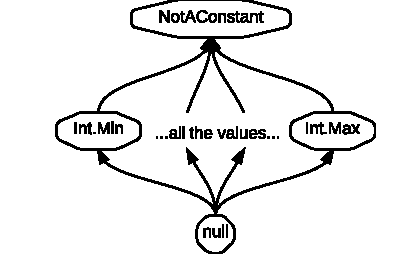
\includegraphics{img/ConstLattice.pdf}  
    \caption{The Lattice for Constant Propagation\label{constlattice}}
\end{figure}        
        
        The transfer function annotates every expression 
        with its constant value if possible. An access to a 
        variable is annotated with this variable's value 
        from the data flow, some expressions can be symbolically 
        executed using the annotations to get operands values, 
        and constants are annotated with their value retrieved 
        from Type Tables.
        
        The data flow is updated only for assignment statement, 
        reference assignment statement and for function call, 
        because some local variables can be passed by reference, 
        which can change their value. The right hand side of 
        the assignment is an expression, which should already by 
        annotated with its value that is used for the data 
        flow value.
        

        

    \section{Type Analysis}
        \note{
        \begin{itemize}
            \item Type Information representation
            \item Data Flow representation
            \item AST annotations
        \end{itemize}}

    \section{The Analyser pipeline and AnalysisDriver}
        \note{Description of the high level public interface 
        and the phases of the full analysis process.}

%pygmentize_options: -O startinline=True
\chapter{Results}

The project has been evaluated on the following open source PHP frameworks and 
websites.

\begin{itemize}
    \item PHPUnit: a port of JUnit unit testing framework for PHP. 
    \item Zend Framework: popular general purpose PHP framework. 
        \note{over 3000 problems reported. Quite a big bite to chew with analysing and categorizing all of them.}
    \item Nette: another popular PHP framework for building websites.
        \note{Findings not so impressive: 1 (probably only) documentation error :(}
    \item Piwik: open source version of Google Analytics. \note{few hundred problems found}
    \item PrestaShop: open source e-commerce solution. \note{few hundred problems found}
    \item Composer: popular dependency management system for PHP libraries. \note{few hundred problems found}
    \item WordPress: on of the most popular content management systems.
\end{itemize}

An evaluation always started with downloading a git repository with the 
latest source code of given PHP project. Than the analysis was run and 
all the discovered problems were collected and categorized.
Actual errors were rectified and recorded as commits in the 
git repository. 

Often one real issue in the source code caused several 
warnings to be reported by the tool. For instance, if a documentation 
of a type of a field was not correct, most the lines where 
a value was assigned to that field were reported, however, the 
root of the cause was actually the only one line with the 
wrong type documentation. Such cases were counted as a 
single problem.

\section{Problems Taxonomy}

The problems were divided into few main categories 
described below. Some of the problems recurring 
across all the projects are discussed in this section, 
while the more project specific problems are 
investigated later each project's section.

\paragraph*{Style:} a category of problems that 
are not directly affecting the functionality of the 
application, but they can be considered as a bad 
coding style. 

\begin{itemize}
    \item[] \textit{Relaying on default return value} -- when an execution of a 
        routine does not end with a return statement, its 
        return value is \code{NULL} by default, which can then 
        be cast to values of other types, like \code{false} 
        for example. Developers rely on this feature and omit 
        the return statement if they want to return \code{NULL} or 
        something that \code{NULL} can be cast to.
\end{itemize}

\paragraph*{Documentation:} inconsistency of the PHPDoc type 
documentation and what the the code does. This category includes 
only cases where it is clear that the documentation is wrong, not the code, 
for example, due to updates in the code that were not reflected 
in the documentation. The inconsistency may also indicate 
another problem, in which case it does not belong to this category. 

Interestingly, most of the inconsistencies of type of a parameter 
of a function call typically lead through several routines that 
only forward the parameter to the next routine until 
eventually the routine that has a wrong documentation is reached.

\begin{itemize}
    \item[] \textit{Missing} \code{false} \textit{in return value type documentation} -- 
        this is common pattern in PHP where a routine returns \code{false} 
        when it fails to do what it was supposed to do. For example, 
        function \code{fopen} returns \code{resource} of \code{false} 
        if the resource could not be opened. It is so common that 
        developers tend to forget to put \code{false} into the documentation.
\end{itemize}

\paragraph*{Actual Error:} includes all problems that can cause 
an unexpected exception or unexpected runtime error or notice.


\paragraph*{False Positive:} problems reported by the tool that 
are not in fact real problems. Includes only false positives 
that cannot be eliminated because of fundamental design reasons 
or are not intended to be eliminated, because it would 
cause some actual positives to be missed.


\begin{itemize}
    \item[] \textit{Unused routine arguments} -- when a method is an override of 
        some base method, it can have the same signature and if some of the 
        parameters are not used, they are not reported. There are however 
        some cases where the routine is implementing some interface by convention 
        that is not explicitly expressed in the syntax of PHP.
        For example, the pre-object-oriented pattern for global functions 
        overriding. In such case the analyzer cannot determine that the unused 
        parameter is in fact a part of an interface. Note that such function 
        could omit the unused parameter and everything would work the same, 
        therefore this may or may not be considered a false positive.
    \item[] \textit{Amendable false positive} -- false positives 
        that are reported, although the algorithm the analyzer 
        is using should not report them. Those indicate errors 
        in the implementation.
    \item[] \textit{Built-in documentation errors} -- false positives 
        due to the inaccuracy of the documentation of built-in 
        functions and classes that was used in the experiment.
\end{itemize}

\section{Summary}

\newcommand{\subcat}[1]{\hspace{0.5cm}\small{\textit{#1}}} 
\newcommand{\reldefret}{\subcat{default return value}}

\newcommand{\sumh}[1]{\textbf{#1}}
%\newcommand{\sumh}[1]{\begin{turn}{60}#1\end{turn}}

\begin{center}
    \begin{tabular}{| p{5cm} | r | r | r | r | r |}
    \hline
    \sumh{Category}         &   \sumh{PHPUnit}      &   \sumh{Zend}       &   \sumh{Nette}    &   \sumh{WP}    &   \sumh{total}   \\ \hline
    Style                   &   6                   &       NA                      &   NA              &   NA                  &   6       \\ \hline
    \reldefret              &   2                   &       NA                      &   NA              &   NA                  &   2       \\ \hline        
    Documentation           &   10                  &       NA                      &   NA              &   NA                  &   10      \\ \hline    
    \subcat{missing false}  &   3                   &       NA                      &   NA              &   NA                  &   3       \\ \hline
    Actual Error            &   1                   &       NA                      &   NA              &   NA                  &   1      \\ \hline    
    False positive          &   8                   &       NA                      &   NA              &   NA                  &   8      \\ \hline    
   \subcat{unused arguments}&   1                   &       NA                      &   NA              &   NA                  &   1      \\ \hline        
    \subcat{amendable}      &   4                   &       NA                      &   NA              &   NA                  &   4      \\ \hline            
 \subcat{built-in doc error}&   3                   &       NA                      &   NA              &   NA                  &   3      \\ \hline
    \textbf{Total} 
    (excl. false positives) &17                   &       NA                      &   NA              &   NA                  &   17      \\ \hline                
    \end{tabular}
\end{center}



\section{PhpUnit}
PHPUnit is a mature and well established project that has been 
developed for more than 6 years by 156 contributors. 
Being a unit testing framework, PHPUnit itself has extensive 
unit test suite. For the experiment the master branch of the clone of the 
repository retrieved on 18.5.2014 was used.

\subsection{Individual Errors.}

\note{Q: move the table to an Appendix? Should I do such table for each project? -- 
lots of data and work to be done. Maybe only for PHPUnit and for other projects only 
discuss interesting errors and provide quantitative data in the summary table above.}

\begin{center}
    \begin{tabular}{| l | l | l | p{6cm} |}
    \hline
    File                             &   Line    &   Category       &   Note  \\ \hline
    \path{Framework\TestCase.php}    &   1722    &   Style          &   Foreach used in form \code{foreach(\$array as \$key=>\$val)} although the \code{\$key} variable was not used anywhere. \\ \hline
    \path{Framework\TestCase.php}    &   1726    &   Style          &   Discussion follows. \\ \hline    
    \path{Framework\Assert.php}      &   1861    &   Actual Error   &   Discussion follows. \\ \hline
    \path{Framework\Assert.php}      &   1960    &   Documentation  &   The routine code allows one of the arguments to be an \code{array} and works with it as such, but the documentation states that it can only be \code{boolean}. \\ \hline        
    \path{Framework\Assert.php}      &   1896    &   Documentation  &   \code{assertSelectEquals} method restricts its parameter type to be \code{integer} and is invoked with \code{boolean}. 
                                                                        However, the parameter value gets only forwarded to \code{convertSelectToTag}, which accepts any type (mixed). \\ \hline    
    \path{Util\XML.php}              &   544     &   Documentation  &   \multirow{2}{6cm}{Missing \code{false} in return value documentation.} \\ \cline{1-3}    
    \path{Util\Test.php}             &   294     &   Documentation  &   \\ \hline
    \path{Util\GlobalState.php}      &   351     &   False Positive &   \multirow{2}{6cm}{Built-in documentation error.} \\ \cline{1-3}    
    \path{Util\Test.php}             &   360     &   False Positive &   \\ \hline
    \path{Framework\TestCase.php}    &   1941    &   Documentation  &   Field \code{mockObjectGenerator} is documented to have type \code{array}, 
                                                                        but value of type \code{MockObject\_Generator} 
                                                                        is assigned to it. The documentation should be updated. \\ \hline
    \path{Util\GlobalState.php}      &   351     &   False Positive &   Built-in documentation error. \\ \hline
    \path{Util\Test.php}             &   46      &   False Positive &   Function \code{trait\_exists} is conditionally declared if it does not exist.
                                                                        It follows the same signature of actual built-in function \code{trait\_exists}, 
                                                                        but it has empty body, therefore it does not use its arguments. \\ \hline
    \end{tabular}
\end{center}


\subsection{Actual Error When Handling \code{DOMElements}}

The error is related to the following code (shortened).

%pygmentize_begin php
% function assertEqualXMLStructure(
%   DOMElement $expectedElement/*, ...*/) {
%   ///...
%   PHPUnit_Util_XML::removeCharacterDataNodes($expectedElement);
%   PHPUnit_Util_XML::removeCharacterDataNodes($actualElement);
%   //...
%   for ($i = 0; $i < $expectedElement->childNodes->length; $i++) {
%       self::assertEqualXMLStructure(
%           $expectedElement->childNodes->item($i) /*<<< error */
%           /*...*/);
% }
%pygmentize_end
\begin{Verbatim}[commandchars=\\\{\}]
 \PY{k}{function} \PY{n+nf}{assertEqualXMLStructure}\PY{p}{(}
   \PY{n+nx}{DOMElement} \PY{n+nv}{\PYZdl{}expectedElement}\PY{c+cm}{/*, ...*/}\PY{p}{)} \PY{p}{\PYZob{}}
   \PY{c+c1}{///...}
   \PY{n+nx}{PHPUnit\PYZus{}Util\PYZus{}XML}\PY{o}{::}\PY{n+na}{removeCharacterDataNodes}\PY{p}{(}\PY{n+nv}{\PYZdl{}expectedElement}\PY{p}{);}
   \PY{n+nx}{PHPUnit\PYZus{}Util\PYZus{}XML}\PY{o}{::}\PY{n+na}{removeCharacterDataNodes}\PY{p}{(}\PY{n+nv}{\PYZdl{}actualElement}\PY{p}{);}
   \PY{c+c1}{//...}
   \PY{k}{for} \PY{p}{(}\PY{n+nv}{\PYZdl{}i} \PY{o}{=} \PY{l+m+mi}{0}\PY{p}{;} \PY{n+nv}{\PYZdl{}i} \PY{o}{\PYZlt{}} \PY{n+nv}{\PYZdl{}expectedElement}\PY{o}{\PYZhy{}\PYZgt{}}\PY{n+na}{childNodes}\PY{o}{\PYZhy{}\PYZgt{}}\PY{n+na}{length}\PY{p}{;} \PY{n+nv}{\PYZdl{}i}\PY{o}{++}\PY{p}{)} \PY{p}{\PYZob{}}
       \PY{n+nx}{self}\PY{o}{::}\PY{n+na}{assertEqualXMLStructure}\PY{p}{(}
           \PY{n+nv}{\PYZdl{}expectedElement}\PY{o}{\PYZhy{}\PYZgt{}}\PY{n+na}{childNodes}\PY{o}{\PYZhy{}\PYZgt{}}\PY{n+na}{item}\PY{p}{(}\PY{n+nv}{\PYZdl{}i}\PY{p}{)} \PY{c+cm}{/*\PYZlt{}\PYZlt{}\PYZlt{} error */}
           \PY{c+cm}{/*...*/}\PY{p}{);}
 \PY{p}{\PYZcb{}}
\end{Verbatim}

The method \code{assertEqualXMLStructure} accepts only instances 
of \code{DOMElement}, but it invokes itself recursively with first 
argument of type \code{DOMNode}. Because according to the 
PHP documentation the value of the \code{childNodes} property 
of interface \code{DOMNode} is an instance of \code{DOMNodeList} 
and the method \code{item(integer)} of \code{DOMNodeList} 
returns \code{DOMNode}, it is a type mismatch error as \code{DOMNode} 
is not subtype of \code{DOMElement}.

In the PHP implementation of DOM model, the only implementations of 
\code{DOMNode} either inherit from \code{DOMElement} or 
implement \code{DOMCharacterData}, and those are removed 
from the \code{childNodes} collection by \code{removeCharacterDataNodes}. 
Therefore, in most cases, this code behaves as expected. 

However, the \code{DOMNode} interface can be implemented by any user 
defined class, which does not have to inherit from 
\code{DOMElement}, and if an instance of such class was present 
in the \code{childNodes} collection, the code would cause an 
exception when trying to invoke \code{assertEqualXMLStructure} 
with an argument of wrong type.

Note that if method \code{removeCharacterDataNodes} removed 
all the child nodes that are not instances of \code{DOMElement}, 
the code would be correct, but the error would still be reported, 
therefore it would be false positive.


\section{Zend Framework}

\section{Nette}

\section{WordPress}



\chapter{Conclusion}

    In this thesis we presented a project with code name 
    Control Flow for Phalanger, which can analyse PHP 
    source code in order to discover type related errors 
    and mismatches with type documentation.
    
    The Control Flow for Phalanger was evaluated on 
    three real world PHP project. Although, the tool 
    does not use heap abstraction and 
    does not perform context sensitive analysis, it was 
    still capable of discovering several real 
    issues with a good ratio of false positives. 
    
    This result may indicate that, were some imprecision 
    in the analysis results can be tolerated, the 
    modular approach we used can give results comparable 
    to those of tools that use more complex methods, with 
    possibly better scalability.

    \section{Future Work}
    
        \subsubsection*{Phalanger Integration}
        The Control Flow for Phalanger has not yet been fully 
        integrated into the Phalanger project. This includes 
        integration with the compiler in order to enable 
        code optimizations and evaluation of the possible 
        performance gain when running PHP websites like WordPress.
        
        \subsubsection*{Arrays Support}
        Array support has not been implemented yet. Variables 
        that can be of type array are analysed properly, but 
        the structure of the array is not analysed. Therefore 
        any time an element of an array is accessed, we do not 
        have any type information for it and have to assume 
        the worst -- it can be any type.
        
        Arrays in PHP are often used as ad-hoc structural 
        types like records in Pascal or structs in C. 
        In such case, the array is typically subscribed to 
        only by a set of known string constants, 
        which represents a good opportunity for 
        static analysis.
        
        One of the possible concepts for local arrays 
        analysis we would like to investigate further 
        is based on the fact that arrays in PHP have 
        copy semantics as opposed to most of the other 
        programming languages. We can model each constant 
        index of an array as a separate local variable. 
        For example, for code \code{\$a['x']=3} we create 
        two local variables: \code{\$a} and \code{\$a@x} 
        and the type of \code{\$a} would be an array and 
        the type of \code{\$a@x} would be an integer. 
        Such representation would still permit us to use 
        bit-vectors as the \emph{data-flow} representation.
        
        \subsubsection*{Performance Evaluation and Tuning}
        Some of the design decisions in Control Flow for 
        Phalanger were made for performance reasons. The 
        design is done an a way that permits further 
        performance targeted improvements, but first 
        an evaluation of the current performance is 
        required.
        
        One of the possible enhancements is more efficient 
        type information representation. Type information 
        is represented using a 64 bit value, however, 
        we can go even further and represent the type 
        information with 8 bit number, which will be an index 
        into a table with all the possible type information 
        instances for one routine. This would give us 255 
        possible combinations of types, which we assume is 
        enough for most of the routines. Since every expression 
        node in AST is annotated with type information and 
        \emph{data-flow} values are arrays of 
        type information, we expect memory consumption 
        and possibly performance improvement.
        
        %\subsubsection*{Context-sensitive Analysis}
        


%%% Seznam použité literatury
\def\bibname{Bibliography}
\addcontentsline{toc}{chapter}{\bibname}
\bibliographystyle{ieeetr}
\bibliography{bibliography}

%%% Tabulky v diplomové práci, existují-li.
\chapwithtoc{List of Tables}


%\begin{center}
    \begin{longtable}{| l | l | l | p{6cm} |}
    
    \hline 
    \textbf{File} &   \textbf{Line}    &   \textbf{Category}       &   \textbf{Note}  \\ \hline 
    \endfirsthead
    
    %\multicolumn{4}{c}{{\bfseries Continued from previous page}} \\
    %\phpunittableheader{}
    \endhead

    %\hline \multicolumn{4}{|r|}{{Continued on next page}} \\ \hline
    \endfoot

    %\hline
    \endlastfoot    
    
    
    \path{F\TestCase.php}    &   1722    &   Style          &   Foreach used in form \code{foreach(\$array as \$key=>\$val)} although the \code{\$key} variable was not used anywhere. \\ \hline
    \path{F\TestCase.php}    &   1726    &   Style          &   \\ \hline    
    \path{F\Assert.php}      &   1861    &   Actual Error   &   Discussion in the \wthesis. \\ \hline
    \path{F\Assert.php}      &   1960    &   Documentation  &   The routine code allows one of the arguments to be an \code{array} and works with it as such, but the documentation states that it can only be \code{boolean}. \\ \hline        
    \path{F\Assert.php}      &   1896    &   Documentation  &   \code{assertSelectEquals} method restricts its parameter type to be \code{integer} and is invoked with \code{boolean}. 
                                                                        However, the parameter value gets only forwarded to \code{convertSelectToTag}, which accepts any type (mixed). \\ \hline    
    \path{U\XML.php}              &   544     &   Documentation  &   \multirow{3}{6cm}{Missing \code{false} in return value documentation.} \\ \cline{1-3}    
    \path{F\TestSuite.php}  &   737     &   Documentation  &   \\ \cline{1-3}        
    \path{U\Test.php}             &   294     &   Documentation  &   \\ \hline
    \path{U\GlobalState.php}      &   351     &   False Positive &   \multirow{4}{6cm}{Built-in documentation error.} \\ \cline{1-3}    
    \path{U\Test.php}             &   360     &   False Positive &   \\ \cline{1-3}
    \path{T\Command.php}        &   791     &   False Positive &   \\ \cline{1-3}
    \path{T\Command.php}        &   745     &   False Positive &   \\ \hline
    \path{F\TestCase.php}    &   1941    &   Documentation  &   Field \code{mockObjectGenerator} is documented to have type \code{array}, 
                                                                        but value of type \code{MockObject\_Generator} 
                                                                        is assigned to it. The documentation should be updated. \\ \hline
    \path{U\Test.php}             &   46      &   False Positive &   Function \code{trait\_exists} is conditionally declared if it does not exist.
                                                                        It follows the same signature of actual built-in function \code{trait\_exists}, 
                                                                        but it has empty body, therefore it does not use its arguments. \\ \hline
    \path{F\C\Count.php} &   90      &  Style &   \multirow{1}{6cm}{Not all paths in a routine return a value.} \\ \cline{1-3}
    \path{F\C\IsType.php} &   127      &  Style &   \\ \hline
    \path{F\C\Count.php} &   100      &  False positive &   \\ \hline
    \path{F\C\Count.php} &   115      &  Documentation &  The documentation of method \code{getCountOf} states that it returns \code{boolean}, but 
                                                                            it returns \code{integer}.\\ \hline                                                     
    \path{F\C\EMessage.php} &   69      &  False positive &   \\ \hline
    \path{F\C\IsAnything.php} &   76      &  False positive &  Unused parameter of a method that implements an interface. \\ \hline
    \path{F\C\IsJson.php} &   88      &  Documentation &  Method \code{determineJsonError} has wrong type documentation for one of its parameters. \\ \hline    
    \path{F\C\Count.php} &   100      &  False positive &   \\ \hline    
    \path{T\Command.php} &   339      &  Style &   Debatable: function \code{ini\_set} expects string, however, anything given to it is implicitly converted to string. \\ \hline
    \path{U\Configuration.php} &   991      &  Documentation &   The documentation of method \code{getInteger} states that the return type is \code{boolean}. \\ \hline
    \path{U\D\Logger.php} &   198      &  Documentation &   Wrong documentation of field's type. \\ \hline
    \path{U\T\ResultPrinter.php} &   206      &  False positive &   \\ \hline
    \end{longtable}
%\end{center}

Note: paths are shortened according to this schema:
\begin{itemize*}
    \item \path{F} -- \path{Framework}
    \item \path{F\C} -- \path{Framework\Constraint}
    \item \path{T} -- \path{TextUI}
    \item \path{U} -- \path{Util}
    \item \path{U\D} -- \path{Util\DeprecatedFeature}
    \item \path{U\T} -- \path{Util\TextDox}
    \item \path{F\C\EMessage.php} -- \path{F\C\ExceptionMessage.php}
\end{itemize*}

%%% Přílohy k diplomové práci, existují-li (různé dodatky jako výpisy programů,
%%% diagramy apod.). Každá příloha musí být alespoň jednou odkazována z vlastního
%%% textu práce. Přílohy se číslují.
\chapwithtoc{Attachments}

\openright
\end{document}
